% !TEX encoding = UTF-8 Unicode
% !TeX TXS-program:compile = txs:///pdflatex/[--shell-escape] 

\documentclass[12pt, twoside]{book}
%***************************************************************************************************

% Podstawowe ustawienia języka, według którego formatowany będzie dokument
%\usepackage[english,polish]{babel}
% \usepackage[english]{babel}
\usepackage[MeX]{polski}

% Pakiet babel dla polskiego języka powoduje konflikt z pakietem amssymb.
% Polecenie '\lll' definiują oba pakiety - porządana jest druga definicja.
% \let\lll\undefined

% W przypadku wielojęzykowości ustawia główny język dokumentu
% \selectlanguage{english}

% Kodowanie dokumentu
\usepackage[utf8]{inputenc} 
% \usepackage[T1]{fontenc} 

% Dowolny rozmiar czcionek, kodowanie znaków
% \usepackage{lmodern}

% Polskie wcięcia akapitów
\usepackage{indentfirst}

% Polskie formatowanie typograficzne
\frenchspacing

% Zapewnia liczne usprawnienia wyświetlania i organizacji matematycznych formuł. 
\usepackage{amsmath}

% Wprowadza rozszerzony zestaw symboli m.in. \leadsto
\usepackage{amssymb}

% Dodatkowa, ,,kręcona'' czcionka matematyczna
\usepackage{mathrsfs}

% Dodatkowe wsparcie dla środowiska mathbb, które nie wspiera domyślnie cyfr (\mathbb{})
%\usepackage{bbold}

% Fixes/improves amsmath
\usepackage{mathtools}

\usepackage{graphicx}
\usepackage{subcaption}


% ***************************************************************************************************
% Kolory  
% ***************************************************************************************************

% Umożliwia kolorowanie poszczególnych komórek tabeli
\usepackage[table, svgnames]{xcolor}% http://ctan.org/pkg/

% Umożliwia łatwą zmianę koloru linii w tabeli
\usepackage{tabu}

\usepackage{longtable}

% Umożliwia rozszerzoną kontrolę nad kolorami.
\usepackage{xcolor}

% Definicje kolorów
\definecolor{lgray}{HTML}{9F9F9F}
\definecolor{dgray}{HTML}{5F5F5F}

% ***************************************************************************************************
% Algorytmy 
% ***************************************************************************************************

% Udostępnia środowisko do konstruowania pseudokodów
\usepackage[ruled,vlined,linesnumbered,longend,algochapter]{algorithm2e}
\renewcommand{\algorithmcfname}{Algorytm}

% Zamiana nazwy środowiska z domyślnej "Algorithm X" na "Pseudokod X"
\newenvironment{algorithm-custom}[1][htb]{ 
	% \renewcommand{\algorithmcfname}{Algorithm}
	\begin{algorithm}[#1]%
	}{
\end{algorithm}
}

% Zmiana rozmiaru komentarzy
\newcommand\algcomment[1]{
	\footnotesize{#1}
}

% Ustawienie zadanego stylu dla komentarzy
\SetCommentSty{algcomment}

% Wyśrodkowana tylda
\usepackage{textcomp}%
\newcommand{\textapprox}{\raisebox{0.5ex}{\texttildelow}}

% Listowanie kodów źródłowych
\usepackage{listings}
\usepackage{xcolor}

% Definicja stylu dla kodu Python
\lstdefinestyle{pythonstyle}{
    language=Python,
    backgroundcolor=\color{gray!10},   % jasnoszare tło
    basicstyle=\ttfamily\small,        % czcionka monospaced, rozmiar small
    keywordstyle=\color{blue}\bfseries, % słowa kluczowe w niebieskim
    commentstyle=\color{green!60!black}\itshape, % komentarze w zielonym italics
    stringstyle=\color{red!70!black},  % ciągi znaków w czerwonym
    numbers=left,                      % numeracja wierszy po lewej
    numberstyle=\tiny\color{gray},     % styl numerów linii
    stepnumber=1,                       % numeruj każdą linię
    numbersep=8pt,                      % odstęp numeracji od kodu
    showstringspaces=false,             % nie pokazuj spacji w stringach
    tabsize=4,                          % tabulacja = 4 spacje
    breaklines=true,                    % łamanie długich linii
    breakatwhitespace=true,             % łam linie w białych znakach
    frame=single,                        % ramka wokół kodu
    rulecolor=\color{black},            % kolor ramki
    captionpos=b                        % podpis pod kodem
}
\renewcommand{\lstlistingname}{Kod źródłowy} % Polska nazwa listingu
% \renewcommand{\lstlistingname}{Source code} % Polska nazwa listingu

% ***************************************************************************************************
% Marginesy 
% ***************************************************************************************************

% Ustawienia rozmiarów stron i ich marginesów
\usepackage[headheight=18pt, top=25mm, bottom=25mm, left=25mm, right=25mm]{geometry}

% Usunięcie górnego marginesu dla środowisk
\makeatletter
\setlength\@fptop{0\p@}	
\makeatother

% ***************************************************************************************************
% Styl 
% ***************************************************************************************************

% Definiuje środowisko 'titlingpage', które zapewnia pełną kontrolę nad układem strony tytułowej.
\usepackage{titling}

% Umożliwia modyfikowanie stylu spisu treści
% \usepackage[subfigure]{tocloft}	
\usepackage{tocloft}	

\tocloftpagestyle{tableOfContentStyle}

% Definiowanie własnych stylów nagłówków i/lub stopek
\usepackage{fancyhdr}

% Domyślny styl dla pracy 
\fancypagestyle{custom}{
	\fancyhf{}									% wyczyść stopki i nagłówki
	\fancyhead[RO]{								% Prawy, nieparzysty nagłówek
		\hrulefill \hspace{16pt} \large Rozdział \thechapter
        %\hrulefill \hspace{16pt} \large Chapter \thechapter
		\put(-471.5,5.5){%
			\makebox(0,0)[l]{%
                \small Politechnika Wrocławska
				%\small Wrocław University of Science and Technology
			}
		}
	}
	\fancyhead[LE]{								% Lewy, parzysty nagłówek
        \large Rozdział \thechapter \hspace{16pt} \hrulefill 
		%\large Chapter \thechapter \hspace{16pt} \hrulefill 
		%\put(-267,5.5){%
        \put(-193,5.5){
			\makebox(0,0)[l]{%
                \small Wydział Informatyki i Telekomunikacji
				%\small Faculty of Information and Communication Technology
			}
		}
	}
	\fancyfoot[LE,RO]{							% Stopki
		\thepage
	}
	\renewcommand{\headrulewidth}{0pt}			% Grubość linii w nagłówku
	\renewcommand{\footrulewidth}{0.2pt}		% Grubość linii w stopce
}

% Domyślny styl dla List of Figures
\fancypagestyle{ListofFiguresStyle}{
	\fancyhf{}									% wyczyść stopki i nagłówki
	\fancyhead[RO]{								% Prawy, nieparzysty nagłówek
		\hrulefill \hspace{16pt} \large Spis rysunków
        %\hrulefill \hspace{16pt} \large List of Figures
		\put(-471.5,5.5){%
			\makebox(0,0)[l]{%
                \small Politechnika Wrocławska
				%\small Wrocław University of Science and Technology
			}
		}
	}
	\fancyhead[LE]{								% Lewy, parzysty nagłówek
		\large Spis rysunków \hspace{16pt} \hrulefill 
        %\large List of Figures \hspace{16pt} \hrulefill 
		%\put(-267,5.5){%
        \put(-193,5.5){
			\makebox(0,0)[l]{%
                \small Wydział Informatyki i Telekomunikacji
				%\small Faculty of Information and Communication Technology
			}
		}
	}
	\fancyfoot[LE,RO]{							% Stopki
		\thepage
	}
	\renewcommand{\headrulewidth}{0pt}			% Grubość linii w nagłówku
	\renewcommand{\footrulewidth}{0.2pt}		% Grubość linii w stopce
}

% Domyślny styl dla List of Tables
\fancypagestyle{ListofTablesStyle}{
	\fancyhf{}									% wyczyść stopki i nagłówki
	\fancyhead[RO]{								% Prawy, nieparzysty nagłówek
		\hrulefill \hspace{16pt} \large Spis tabel
        % \hrulefill \hspace{16pt} \large List of Tables
		\put(-471.5,5.5){%
			\makebox(0,0)[l]{%
                \small Politechnika Wrocławska
				%\small Wrocław University of Science and Technology
			}
		}
	}
	\fancyhead[LE]{								% Lewy, parzysty nagłówek
		\large Spis tabel \hspace{16pt} \hrulefill 
        % \large List of Tables \hspace{16pt} \hrulefill 
		%\put(-267,5.5){%
        \put(-193,5.5){
			\makebox(0,0)[l]{%
                \small Wydział Informatyki i Telekomunikacji
				%\small Faculty of Information and Communication Technology
			}
		}
	}
	\fancyfoot[LE,RO]{							% Stopki
		\thepage
	}
	\renewcommand{\headrulewidth}{0pt}			% Grubość linii w nagłówku
	\renewcommand{\footrulewidth}{0.2pt}		% Grubość linii w stopce
}


% Domyślny styl dla bibliografii
\fancypagestyle{bibliographyStyle}{
	\fancyhf{}									% wyczyść stopki i nagłówki
	\fancyhead[RO]{								% Prawy, nieparzysty nagłówek
		\hrulefill \hspace{16pt} \large Bibliografia
        % \hrulefill \hspace{16pt} \large Bibliography
		\put(-471.5,5.5){%
			\makebox(0,0)[l]{%
				\small Politechnika Wrocławska
				%\small Wrocław University of Science and Technology
			}
		}
	}
	\fancyhead[LE]{								% Lewy, parzysty nagłówek
		\large Bibliografia \hspace{16pt} \hrulefill 
        % \large Bibliography \hspace{16pt} \hrulefill 
		%\put(-267,5.5){%
        \put(-193,5.5){
			\makebox(0,0)[l]{%
                \small Wydział Informatyki i Telekomunikacji
				%\small Faculty of Information and Communication Technology
			}
		}
	}
	\fancyfoot[LE,RO]{							% Stopki
		\thepage
	}
	\renewcommand{\headrulewidth}{0pt}			% Grubość linii w nagłówku
	\renewcommand{\footrulewidth}{0.2pt}		% Grubość linii w stopce
}

% Domyślny styl dla dodatków
\fancypagestyle{appendixStyle}{
	\fancyhf{}									% wyczyść stopki i nagłówki
	\fancyhead[RO]{								% Prawy, nieparzysty nagłówek
		\hrulefill \hspace{16pt} \large Dodatek \thechapter
        % \hrulefill \hspace{16pt} \large Appendix \thechapter
		\put(-472.1, 12.1){%
			\makebox(0,0)[l]{%
				\includegraphics[width=0.05\textwidth]{resources/pwr-logo}
			}
		}
		\put(-443,5.5){%
			\makebox(0,0)[l]{%
				\small Politechnika Wrocławska
				%\small Wrocław University of Science and Technology
			}
		}
	}
	\fancyhead[LE]{								% Lewy, parzysty nagłówek
		\large Dodatek \thechapter \hspace{16pt} \hrulefill 
        %\large Appendix \thechapter \hspace{16pt} \hrulefill 
		\put(-22, 12.1){%
			\makebox(0,0)[l]{%
				\includegraphics[width=0.05\textwidth]{wiz-logo}
			}
		}%
		%\put(-220,5.5){%
		\put(-146,5.5){
			\makebox(0,0)[l]{%
                \small Wydział Informatyki i Telekomunikacji
				%\small Faculty of Information and Communication Technology
			}
		}
	}
	\fancyfoot[LE,RO]{							% Stopki
		\thepage
	}
	\renewcommand{\headrulewidth}{0pt}			% Grubość linii w nagłówku
	\renewcommand{\footrulewidth}{0.2pt}		% Grubość linii w stopce
}


% Osobny styl dla stron zaczynających rozdział/spis treści itd. (domyślnie formatowane jako "plain")
\fancypagestyle{chapterBeginStyle}{
	\fancyhf{}%
	\fancyfoot[LE,RO]{
		\thepage
	}
	\renewcommand{\headrulewidth}{0pt}
	\renewcommand{\footrulewidth}{0.2pt}
}

% Styl dla pozostałych stron spisu treści
\fancypagestyle{tableOfContentStyle}{
	\fancyhf{}%
	\fancyfoot[LE,RO]{
		\thepage
	}
	\renewcommand{\headrulewidth}{0pt}
	\renewcommand{\footrulewidth}{0.2pt}
}

% Formatowanie tytułów rozdziałów i/lub sekcji
\usepackage{titlesec}


% Formatowanie tytułów rozdziałów
\titleformat{\chapter}[hang]
{\normalfont\Huge\bfseries}
{\thechapter.}
{1ex}
{}
\titlespacing*{\chapter}{0pt}{-35pt}{18pt}

% Formatowanie tytułów sekcji
\titleformat{\section}[hang]
{\normalfont\Large\bfseries}											
{\thesection.}
{1ex}
{} 

\titleformat{\subsection}[hang]
{\normalfont\large\bfseries}											
{\thesubsection.}
{1ex}
{} 
% formatowanie elementów przed modyfikowanym tytułem


% ***************************************************************************************************
% Linki
% ***************************************************************************************************

% Umożliwia wstawianie hiperłączy do dokumentu
\usepackage{hyperref}							% Aktywuje linki

\hypersetup{
	colorlinks	=	true,					% Koloruje tekst zamiast tworzyć ramki.
	linkcolor	=	blue,					% Kolory: referencji,
    citecolor	=	blue,					% cytowań,
	urlcolor	=	blue					% hiperlinków.
}

% Do stworzenia hiperłączy zostanie użyta ta sama (same) czcionka co dla reszty dokumentu
\urlstyle{same}


% ***************************************************************************************************
% Linki
% ***************************************************************************************************

% Umożliwia zdefiniowanie własnego stylu wyliczeniowego
\usepackage{enumitem}

% Nowa lista numerowana z trzema poziomami
\newlist{myitemize}{itemize}{3}

% Definicja wyglądu znacznika pierwszego poziomu
\setlist[myitemize,1]{
	label		=	\textbullet,
	leftmargin	=	4mm}

% Definicja wyglądu znacznika drugiego poziomu
\setlist[myitemize,2]{
	label		=	$\diamond$,
	leftmargin	=	8mm}

% Definicja wyglądu znacznika trzeciego poziomu
\setlist[myitemize,3]{
	label		=	$\diamond$,
	leftmargin	=	12mm
}

% ***************************************************************************************************
% Inne pakiety
% ***************************************************************************************************

% Dołączanie rysunków
\usepackage{graphicx}

% Figury i przypisy
\usepackage{caption}
\usepackage{subcaption}

% Umożliwia tworzenie przypisów wewnątrz środowisk
\usepackage{footnote}

% Umożliwia tworzenie struktur katalogów
\usepackage{dirtree}

% Rozciąganie komórek tabeli na wiele wierszy
\usepackage{multirow}

% Precyzyjne obliczenia szerokości/wysokości dowolnego fragmentu wygenerowanego przez LaTeX
\usepackage{calc}

% ***************************************************************************************************
% Matematyczne skróty
% ***************************************************************************************************

% Skrócony symbol liczb rzeczywistych
\newcommand{\RR}{\mathbb{R}}

% Skrócony symbol liczb naturalnych
\newcommand{\NN}{\mathbb{N}}

% Skrócony symbol liczb wymiernych
\newcommand{\QQ}{\mathbb{Q}}

% Skrócony symbol liczb całkowitych
\newcommand{\ZZ}{\mathbb{Z}}

% Skrócony symbol logicznej implikacji
\newcommand{\IMP}{\rightarrow}

% Skrócony symbol  logicznej równoważności
\newcommand{\IFF}{\leftrightarrow}

% ***************************************************************************************************
% Środowiska
% ***************************************************************************************************

% Środowisko do twierdzeń
\newtheorem{theorem}{Twierdzenie}[chapter]

% Środowisko do lematów
\newtheorem{lemma}{Lemat}[chapter]

% Środowisko do przykładów
\newtheorem{example}{Przykład}[chapter]

% Środowisko do wniosków
\newtheorem{corollary}{Wniosek}[chapter]

% Środowisko do definicji
\newtheorem{definition}{Definicja}[chapter]

% Środowisko do dowodów
\newenvironment{proof}{
	\par\noindent \textbf{Dowód.}
}{
\begin{flushright}
	\vspace*{-6mm}\mbox{$\blacklozenge$}
\end{flushright}
}

% Środowisko do uwag
\newenvironment{remark}{
	\bigskip \par\noindent \small \textbf{Uwaga.}
}{
\begin{small}
	\vspace*{4mm}
\end{small}
}

% dodatkowe pomagające, oczywiście nie wszystskie są wymagane
\usepackage{psfrag}
\usepackage{amsfonts}
\usepackage{supertabular}
\usepackage{array}
\usepackage{tabularx}
\usepackage{hhline}
\usepackage{minted}
\usepackage{xurl}
\usepackage{microtype}
\usepackage{booktabs} % for professional tables
\usepackage{makecell}
\usepackage{rotating}
\usepackage{multicol}
\usepackage{cuted}
\usepackage{colortbl}
\usepackage{adjustbox}
\usepackage{color,soul}
% \usepackage{subfigure}
\usepackage{pdfpages}

\let\cleardoublepage\clearpage

\usepackage{pifont}
\newcommand{\cmark}{\ding{51}}
\newcommand{\xmark}{\ding{55}}
\newcommand{\bftab}{\fontseries{b}\selectfont}

\newcolumntype{P}[1]{>{\raggedright\arraybackslash\noindent}p{#1}}


\newcolumntype{R}[1]{>{\raggedleft\arraybackslash}p{#1}}
\newcolumntype{L}[1]{>{\raggedright\arraybackslash}p{#1}}
\newcolumntype{C}[1]{>{\centering\arraybackslash}m{#1}}

\usepackage{caption}
\usepackage[nocompress]{cite}
\usepackage{url}
\usepackage{color,soul}
\usepackage{svg}
\usepackage{tabto}
\usepackage{wrapfig}

% formatowanie pierwszych stron rozdziałów - pomagające
\newcommand{\resetformatting}{ 
\fancypagestyle{plain}{
    	\fancyhf{}%
    	\fancyfoot[LE,RO]{
    		\thepage
    	}
    	\renewcommand{\headrulewidth}{0pt}
    	\renewcommand{\footrulewidth}{0.2pt}
    } }
\newcommand{\doublepage}{ 
\newpage
\thispagestyle{empty}
\cleardoublepage}

\newcommand\Chapter[1]{ 
\chapter{#1}
\thispagestyle{chapterBeginStyle}}

%***************************************************************************************************
% Wlasne komendy
% ***************************************************************************************************
\newcommand{\kgMargin} [1]{\marginpar{\color{magenta} {\bf PP}: \small{#1}}}
\newcommand{\kg}[1]{{\color{magenta} {\bf PP}: \small{#1}}}

\newcommand{\rrMargin} [1]{\marginpar{\color{magenta} {\bf RR}: \small{#1}}}
\newcommand{\rr}[1]{{\color{blue} {\bf RR}: \small{#1}}}

% Dodac reszte komentarzy od reszty osob - niech kazdy wybierze sobie kolor

% Numerowanie linii w drafcie
% \usepackage{lineno}
% \renewcommand\linenumberfont{\normalfont\scriptsize}
% \linenumbers

\frontmatter

\title{\textbf{Projektowanie bezpiecznej architektury ICT - Projekt}}
\author{
Pola Polańska 276087, Piotr Bonar 272720, Kacper Kurp 268555,\\
Wiktor Szajerka 272432, Roch Szewczyk 263828, Robert Rubaszek 272372
}
\date{Czerwiec 2026}

% Ten plik jest wyłącznie do podpinania kolejnych rozdziałów
\begin{document}
\raggedbottom
\maketitle
\doublepage

% Add table of contents
\pagestyle{tableOfContentStyle}
\tableofcontents 

\pagestyle{custom}
\mainmatter
 
% Create chapters:
\Chapter{Opis problemu i analiza obecnej sytuacji}\label{chapter:problem_analysis}

\section{Kontekst projektu}
\subsection{Cyfryzacja ochrony zdrowia w Unii Europejskiej}
W ostatnich latach cyfryzacja stała się jednym z głównych kierunków rozwoju systemów ochrony zdrowia w krajach Unii Europejskiej. Rozwiązania z zakresu eHealth są stopniowo wdrażane zarówno w dużych szpitalach, jak i mniejszych placówkach medycznych, a elektroniczna dokumentacja medyczna zaczyna pełnić rolę podstawowego źródła informacji o pacjencie. Proces ten jest częścią szerszej strategii transformacji cyfrowej UE, której celem jest zwiększenie dostępności usług publicznych oraz poprawa jakości funkcjonowania instytucji ochrony zdrowia \cite{EU_eHealth_2024}.

Jednym z najważniejszych założeń programu „Digital Decade 2030” jest zapewnienie wszystkim obywatelom Unii Europejskiej dostępu do elektronicznej dokumentacji medycznej do roku 2030 \cite{EU_eHealth_2024}. W związku z tym państwa członkowskie rozwijają centralne systemy umożliwiające przechowywanie i udostępnianie danych zdrowotnych w formie cyfrowej. Według raportu „2024 Digital Decade eHealth Indicator Study” średni poziom rozwoju usług eHealth w krajach UE osiągnął w 2023 roku wartość 79\%, co oznacza dalszy wzrost względem poprzednich lat \cite{EU_eHealth_2024}. Polska została wskazana jako jedno z państw o wysokim poziomie dojrzałości cyfrowych usług zdrowotnych, osiągając wynik 90\% \cite{EU_eHealth_2024}.

Raport pokazuje również, że większość państw Unii Europejskiej wykorzystuje scentralizowane platformy dostępu do danych medycznych, a coraz większa liczba usług dostępna jest zarówno przez portale internetowe, jak i aplikacje mobilne \cite{EU_eHealth_2024}. Oznacza to, że współczesne systemy ochrony zdrowia odchodzą od modelu opartego wyłącznie na dokumentacji papierowej i stopniowo przechodzą do środowiska cyfrowego, w którym informacje mogą być dostępne w czasie rzeczywistym dla uprawnionych użytkowników.

Rozwój systemów eHealth wynika również z potrzeby usprawnienia przepływu informacji pomiędzy różnymi jednostkami ochrony zdrowia. W raportach UE podkreśla się, że cyfrowe systemy medyczne mają poprawiać dostęp do danych, wspierać ciągłość leczenia oraz zwiększać zaangażowanie pacjentów w proces opieki zdrowotnej \cite{EU_eHealth_2024}. Szczególnie istotne staje się zapewnienie możliwości szybkiego dostępu do wyników badań, historii leczenia oraz danych dotyczących terapii i przyjmowanych leków.

Pomimo dynamicznego rozwoju technologii wiele krajów nadal mierzy się z problemami związanymi z interoperacyjnością systemów, integracją danych oraz dostępnością niektórych typów dokumentacji medycznej \cite{EU_eHealth_2024}. Raport wskazuje między innymi, że część danych, takich jak obrazy medyczne czy informacje dotyczące implantów, nadal nie jest powszechnie dostępna dla obywateli w formie elektronicznej \cite{EU_eHealth_2024}. Istotnym wyzwaniem pozostaje również zapewnienie odpowiedniego poziomu bezpieczeństwa danych, zgodności z regulacjami UE oraz dostępu wyłącznie dla uprawnionych osób.

Cyfryzacja ochrony zdrowia wiąże się także z koniecznością uwzględnienia potrzeb różnych grup społecznych. W dokumentach UE podkreśla się znaczenie tworzenia systemów dostępnych dla osób starszych, osób z ograniczonymi kompetencjami cyfrowymi oraz użytkowników wymagających dodatkowego wsparcia technicznego \cite{EU_eHealth_2024}. Z tego powodu nowoczesne systemy medyczne powinny być projektowane nie tylko jako zaawansowane technologicznie rozwiązania, ale również jako narzędzia intuicyjne, czytelne i możliwie proste w codziennym użytkowaniu.

\subsection{Cel i założenia projektu}

Projekt dotyczy stworzenia zintegrowanego systemu wspierającego zarządzanie informacjami o pacjentach w Szpitalu im. Bajgla we Wrocławiu. Placówka planuje wdrożenie rozwiązania umożliwiającego gromadzenie, aktualizowanie oraz udostępnianie dokumentacji medycznej w ramach jednego spójnego środowiska cyfrowego. Głównym celem projektu jest usprawnienie przepływu informacji pomiędzy oddziałami oraz ograniczenie problemów wynikających z funkcjonowania dokumentacji papierowej.

Założeniem projektu jest stworzenie systemu umożliwiającego personelowi medycznemu szybki dostęp do najważniejszych informacji o pacjencie, historii leczenia, wyników badań oraz aktualnych zleceń medycznych. Rozwiązanie ma wspierać codzienną pracę lekarzy, pielęgniarek, laboratoriów i administracji poprzez uporządkowanie obiegu danych oraz ograniczenie konieczności ręcznego przekazywania dokumentacji pomiędzy oddziałami.

Projekt uwzględnia również potrzeby pacjentów związane z łatwiejszym dostępem do własnej dokumentacji medycznej oraz możliwością sprawdzania wyników badań w formie elektronicznej. System ma poprawić komunikację pomiędzy placówką a pacjentem oraz ograniczyć konieczność korzystania z dokumentacji papierowej.

Jednym z kluczowych założeń projektu jest także zapewnienie wysokiego poziomu bezpieczeństwa danych medycznych. System powinien umożliwiać kontrolę dostępu do informacji, rozdzielenie uprawnień użytkowników oraz ochronę danych zgodnie z obowiązującymi regulacjami dotyczącymi prywatności i bezpieczeństwa informacji w Unii Europejskiej. Ważnym aspektem projektu pozostaje również stworzenie rozwiązania intuicyjnego i prostego w codziennym użytkowaniu, tak aby ograniczyć problemy związane z wdrażaniem nowych technologii w środowisku szpitalnym.
\section{Analiza obecnej sytuacji}
Szpital im. Bajgla we Wrocławiu jest dużą, wielooddziałową placówką medyczną. W strukturze szpitala znajdują się między innymi oddziały chirurgiczne, interna, neurologia, ortopedia, onkologia, pediatria, oddział intensywnej terapii, Szpitalny Oddział Ratunkowy, laboratorium diagnostyczne, pracownia diagnostyki obrazowej oraz prosektorium. Ze względu na skalę działalności placówka każdego dnia obsługuje dużą liczbę pacjentów, co wiąże się z koniecznością ciągłego przetwarzania i przekazywania ogromnej ilości informacji medycznych pomiędzy różnymi działami szpitala.

Obecnie dokumentacja medyczna w Szpitalu im. Bajgla prowadzona jest głównie w formie papierowej. Karty pacjentów, wyniki badań, opisy diagnostyczne, zlecenia lekarskie, raporty pielęgniarskie oraz dokumenty administracyjne przechowywane są fizycznie i przekazywane pomiędzy oddziałami ręcznie przez personel medyczny lub administracyjny. Powoduje to sytuacje, w których dostęp do informacji jest ograniczony czasowo i zależy od aktualnego miejsca przechowywania dokumentacji. W praktyce oznacza to, że personel często musi samodzielnie odnajdywać potrzebne dokumenty, kontaktować się z innymi działami lub oczekiwać na dostarczenie wyników badań i raportów.

Szczególnie problematyczny jest przepływ informacji pomiędzy oddziałami a laboratorium i diagnostyką obrazową. Wyniki badań laboratoryjnych oraz opisy badań obrazowych przekazywane są w sposób tradycyjny, co wydłuża czas obiegu dokumentacji i utrudnia bieżący dostęp do aktualnych danych pacjenta. Stanowi to krytyczny problem w sytuacjach wymagających szybkiej reakcji.

Brak centralnego systemu cyfrowego powoduje również problemy związane z archiwizacją dokumentacji. Dane pacjentów przechowywane są w wielu segregatorach, kartotekach i archiwach papierowych, przez co odnalezienie starszej historii leczenia może wymagać dużej ilości czasu. W przypadku pacjentów hospitalizowanych wielokrotnie personel musi ręcznie przeszukiwać dokumentację z poprzednich pobytów, aby uzyskać pełny obraz przebiegu leczenia.

Obecny sposób funkcjonowania placówki wpływa bezpośrednio na codzienną pracę lekarzy, pielęgniarek oraz pracowników administracyjnych. Znaczna część czasu poświęcana jest nie na kontakt z pacjentem, lecz na organizację dokumentacji, przekazywanie danych oraz uzupełnianie formularzy papierowych. W wielu przypadkach te same informacje przepisywane są kilkukrotnie do różnych dokumentów, co zwiększa ryzyko błędów i nieścisłości. Problem nasila się szczególnie podczas dużego obciążenia oddziałów lub nagłych sytuacji wymagających szybkiego dostępu do informacji o stanie zdrowia pacjenta.

Chaos informacyjny widoczny jest także z perspektywy pacjentów. Osoby hospitalizowane nie mają bezpośredniego dostępu do swoich wyników badań ani informacji o przebiegu leczenia. Uzyskanie dokumentacji wymaga kontaktu z personelem lub odbioru dokumentów w formie papierowej.

Dodatkowym wyzwaniem jest rosnąca liczba danych medycznych generowanych każdego dnia przez szpital. Rozwój diagnostyki, większa liczba wykonywanych badań oraz rosnąca liczba pacjentów powodują, że tradycyjny model przechowywania dokumentacji staje się coraz mniej efektywny organizacyjnie. Obecny sposób pracy nie odpowiada również kierunkowi rozwoju nowoczesnej ochrony zdrowia w Unii Europejskiej, w której coraz większy nacisk kładzie się na cyfryzację usług medycznych, szybki dostęp do danych oraz integrację informacji o pacjencie \cite{EU_eHealth_2024}.

Analiza obecnej sytuacji pokazuje, że głównym problemem Szpitala im. Bajgla jest brak jednego, centralnego środowiska umożliwiającego sprawne zarządzanie dokumentacją medyczną i przepływem informacji pomiędzy użytkownikami. 
\subsection{Perspektywa dyrektora i organizacji szpitala}

Dyrekcja Szpitala im. Bajgla dostrzega, że obecny sposób organizacji dokumentacji medycznej przestaje być wystarczający dla placówki o tak dużej skali działalności. Wraz ze wzrostem liczby pacjentów oraz ilości wykonywanych badań coraz trudniejsze staje się skuteczne zarządzanie przepływem informacji. Z perspektywy dyrektora szczególnie istotne staje się usprawnienie organizacji pracy i ograniczenie sytuacji, w których personel medyczny poświęca znaczną część czasu na czynności administracyjne.

Istotnym problemem dla organizacji szpitala jest także brak jednolitego standardu pracy z dokumentacją medyczną. Poszczególne oddziały wypracowały własne sposoby przekazywania informacji i organizowania dokumentów, przez co przepływ danych nie jest spójny w całej placówce.

Dyrekcja szpitala zwraca również uwagę na rosnące wymagania związane z dalszą cyfryzacją ochrony zdrowia w Unii Europejskiej. Placówka musi stopniowo dostosowywać się do nowych standardów dotyczących elektronicznej dokumentacji medycznej, bezpieczeństwa danych oraz dostępności usług cyfrowych dla pacjentów \cite{EU_eHealth_2024}.

Dyrekcja oczekuje rozwiązania, które pozwoli personelowi szybciej uzyskiwać dostęp do danych pacjentów, monitorować przebieg leczenia oraz ograniczyć problemy wynikające z opóźnionego przekazywania dokumentacji. Szczególne znaczenie ma to w przypadku oddziałów o dużej dynamice pracy, takich jak SOR czy oddział intensywnej terapii, gdzie szybki dostęp do informacji może mieć bezpośredni wpływ na bezpieczeństwo pacjentów.

Jednocześnie dyrekcja jest świadoma, że wdrożenie nowego systemu będzie dużą zmianą organizacyjną dla całego szpitala. Istnieje obawa, że nieodpowiednio zaprojektowane rozwiązanie mogłoby zwiększyć liczbę obowiązków administracyjnych lub spotkać się z oporem części pracowników. 
\subsection{Perspektywa personelu medycznego}
Personel medyczny Szpitala im. Bajgla należy do grupy użytkowników, na których obecny sposób organizacji dokumentacji wpływa najbardziej bezpośrednio. Lekarze, pielęgniarki, ratownicy medyczni, technicy laboratoryjni oraz pracownicy diagnostyki każdego dnia uczestniczą w procesie przekazywania dużej ilości informacji dotyczących pacjentów. 

Z perspektywy lekarzy jednym z największych problemów jest brak szybkiego dostępu do pełnej historii leczenia pacjenta. Uzyskanie wszystkich potrzebnych informacji wymaga często przeglądania wielu dokumentów, kontaktowania się z innymi oddziałami lub oczekiwania na dostarczenie wyników badań. Lekarze zwracają uwagę, że czas poświęcany na organizację dokumentacji ogranicza możliwość skupienia się bezpośrednio na pracy z pacjentem.

Podobne problemy dotyczą personelu pielęgniarskiego, który oprócz obowiązków związanych z opieką nad pacjentami odpowiada również za prowadzenie i aktualizowanie części dokumentacji medycznej. Powoduje to dodatkowe obciążenie organizacyjne oraz zwiększa ryzyko pomyłek wynikających z nieczytelnych zapisów, zagubionych dokumentów lub nieaktualnych danych.

Istotnym problemem dla personelu jest również przepływ informacji dotyczących badań laboratoryjnych i diagnostycznych. Pracownicy laboratoriów oraz diagnostyki obrazowej wykonują dużą liczbę badań, jednak przekazywanie wyników w tradycyjnej formie wydłuża cały proces komunikacji. Personel medyczny nie posiada możliwości bieżącego monitorowania statusu badań, przez co konieczne staje się wielokrotne sprawdzanie dostępności wyników lub kontaktowanie się z innymi działami szpitala. 

Część pracowników obawia się cyfryzacji placówki. Wśród najczęściej pojawiających się problemów znajdują się obawy przed koniecznością nauki nowych systemów, zmiany dotychczasowych przyzwyczajeń oraz zwiększenia liczby obowiązków administracyjnych. Niektórzy pracownicy postrzegają wdrożenie nowego rozwiązania jako potencjalne utrudnienie codziennej pracy, szczególnie jeśli system byłby skomplikowany. Widoczny jest również strach przed popełnianiem błędów podczas korzystania z nowych narzędzi cyfrowych.

Jednocześnie część personelu dostrzega korzyści wynikające z wprowadzenia centralnego systemu informatycznego. Lekarze i pielęgniarki wskazują przede wszystkim potrzebę szybkiego dostępu do dokumentacji, łatwiejszego przekazywania informacji oraz ograniczenia ilości pracy papierowej. Personel oczekuje rozwiązania, które pozwoli uprościć codzienne obowiązki, zmniejszyć liczbę powtarzalnych czynności administracyjnych oraz usprawnić komunikację pomiędzy oddziałami.

Z punktu widzenia użytkowników bardzo ważna staje się intuicyjność systemu. Nowe rozwiązanie powinno być możliwie proste i czytelne. System nie może wymagać skomplikowanej obsługi ani dużej liczby dodatkowych działań podczas wykonywania podstawowych obowiązków. Istotne znaczenie ma również mobilność rozwiązania, szczególnie w przypadku pracy na oddziałach oraz podczas przemieszczania się pomiędzy pacjentami. Możliwość szybkiego dostępu do danych z poziomu urządzeń mobilnych mogłaby znacząco usprawnić organizację pracy personelu.

Pracownicy oczekują rozwiązania, które rzeczywiście uprości wykonywanie obowiązków, ograniczy chaos organizacyjny oraz poprawi komunikację pomiędzy oddziałami, a nie kolejnego systemu zwiększającego poziom skomplikowania pracy.
\subsection{Perspektywa pacjenta}
Pacjenci Szpitala im. Bajgla są grupą bezpośrednio odczuwającą skutki problemów związanych z organizacją dokumentacji w placówce. Obecny model funkcjonowania szpitala sprawia, że pacjent ma ograniczony dostęp do danych dotyczących własnego leczenia oraz przebiegu hospitalizacji. Uzyskanie wyników badań, historii leczenia czy informacji o dalszych etapach terapii wymaga najczęściej kontaktu z personelem lub odbioru dokumentów w formie papierowej.
Szczególnie problematyczne staje się to w przypadku pacjentów korzystających z usług kilku oddziałów jednocześnie lub wymagających długotrwałego leczenia. Informacje dotyczące badań, konsultacji oraz zaleceń lekarskich są rozproszone, przez co pacjent często nie posiada pełnego obrazu własnego procesu leczenia. Z perspektywy pacjentów ważnym problemem jest czas oczekiwania na informacje. Odbiór wyników badań lub dokumentacji wymaga często osobistej wizyty w szpitalu albo długiego oczekiwania na przekazanie danych przez personel. W praktyce utrudnia to kontakt pacjenta z własną dokumentacją medyczną oraz ogranicza możliwość szybkiego reagowania na zmiany związane ze stanem zdrowia.

Pacjenci zwracają również uwagę na brak przejrzystości procesu leczenia. Osoby hospitalizowane nie zawsze wiedzą, na jakim etapie znajdują się wykonane badania, kiedy pojawią się wyniki oraz jakie działania będą realizowane w dalszej kolejności.
Jednocześnie pacjenci coraz częściej oczekują rozwiązań cyfrowych podobnych do tych wykorzystywanych w innych usługach publicznych i prywatnych. Możliwość sprawdzenia wyników badań online, łatwiejszy kontakt z placówką oraz szybszy dostęp do dokumentacji medycznej postrzegane są jako istotne udogodnienia poprawiające komfort korzystania z opieki zdrowotnej. W raportach dotyczących rozwoju eHealth podkreśla się, że zwiększenie dostępu obywateli do własnych danych medycznych stanowi jeden z głównych kierunków rozwoju nowoczesnej ochrony zdrowia \cite{EU_eHealth_2024}.
\subsection{Bezpieczeństwo danych i dostęp}
Jednym z najważniejszych wyzwań związanych z funkcjonowaniem Szpitala im. Bajgla jest zapewnienie odpowiedniego poziomu bezpieczeństwa dokumentacji medycznej oraz kontrola dostępu do informacji o pacjentach. Dane zdrowotne należą do kategorii danych szczególnie wrażliwych, dlatego sposób ich przechowywania, przetwarzania oraz udostępniania wymaga zachowania wysokich standardów bezpieczeństwa i zgodności z obowiązującymi regulacjami prawnymi.

W obecnym modelu dostęp do danych zależy od fizycznej lokalizacji dokumentów. Taki model utrudnia skuteczną kontrolę nad tym, kto w danym momencie korzysta z dokumentacji oraz czy wszystkie informacje są odpowiednio zabezpieczone przed nieuprawnionym dostępem. Problem staje się szczególnie widoczny w dużej placówce, gdzie każdego dnia z dokumentacją pracuje wiele osób.

Istotnym zagrożeniem jest również możliwość zagubienia dokumentów lub ich nieprawidłowego przekazania pomiędzy oddziałami. Dokumentacja papierowa może zostać przypadkowo pozostawiona w niewłaściwym miejscu, przekazana nieodpowiedniej osobie lub ulec uszkodzeniu.

Z perspektywy organizacji szpitala ważne staje się również rozdzielenie poziomów dostępu do danych. Poszczególni pracownicy nie potrzebują dostępu do wszystkich informacji znajdujących się w dokumentacji medycznej. Lekarze, pielęgniarki, laboranci, administracja czy pracownicy prosektorium korzystają z różnych zakresów danych związanych z wykonywanymi obowiązkami. W obecnym modelu papierowym kontrola takich uprawnień jest utrudniona, ponieważ dokumentacja może być fizycznie przekazywana pomiędzy wieloma osobami bez możliwości dokładnego monitorowania dostępu.

Ważnym aspektem są również wymagania wynikające z regulacji obowiązujących na terenie Unii Europejskiej. Cyfrowe systemy ochrony zdrowia muszą być zgodne między innymi z zasadami GDPR dotyczącymi ochrony danych osobowych oraz bezpieczeństwa informacji \cite{EU_eHealth_2024}. Oznacza to konieczność zapewnienia odpowiedniego uwierzytelniania użytkowników, kontroli dostępu do dokumentacji oraz możliwości monitorowania działań wykonywanych w systemie. 
Istotnym wyzwaniem pozostaje również zapewnienie bezpieczeństwa przy jednoczesnym zachowaniu prostoty użytkowania systemu. Personel medyczny pracuje pod dużą presją czasu, dlatego procedury związane z logowaniem i dostępem do danych nie mogą nadmiernie utrudniać codziennej pracy.
\subsection{Problemy techniczne i organizacyjne}
Planowana cyfryzacja Szpitala im. Bajgla wiąże się nie tylko z koniecznością stworzenia nowego systemu informatycznego, ale również z dużą zmianą organizacyjną obejmującą sposób funkcjonowania całej placówki. Ze względu na skalę szpitala oraz liczbę oddziałów wdrożenie nowego rozwiązania wymaga uwzględnienia wielu problemów technicznych, logistycznych i organizacyjnych, które mogą wpływać na późniejsze działanie systemu oraz jego akceptację przez użytkowników.

Jednym z głównych wyzwań jest konieczność zaprojektowania systemu dostosowanego do pracy wielu różnych działów szpitala jednocześnie. Każdy oddział funkcjonuje w nieco inny sposób i posiada własne potrzeby związane z dokumentacją oraz przepływem informacji. Oznacza to, że system musi być wystarczająco elastyczny, aby umożliwić obsługę różnych procesów medycznych bez nadmiernego komplikowania interfejsu użytkownika.

Istotnym problemem technicznym jest również stworzenie odpowiedniej infrastruktury umożliwiającej funkcjonowanie systemu w całym szpitalu. Placówka wymaga stabilnego dostępu do sieci, odpowiednich urządzeń dla personelu medycznego oraz bezpiecznego środowiska przechowywania danych. 
Wdrożenie systemu obejmującego wiele oddziałów oznacza konieczność zapewnienia ciągłości działania nawet w przypadku awarii części infrastruktury lub problemów technicznych. 

Ważnym wyzwaniem jest także przeniesienie istniejącej dokumentacji papierowej do nowego środowiska cyfrowego. Szpital posiada dużą ilość archiwalnych danych dotyczących pacjentów, które przez lata były przechowywane w formie tradycyjnej. Proces cyfryzacji dokumentacji wymaga więc ustalenia sposobu migracji danych, określenia priorytetów oraz przygotowania procedur umożliwiających stopniowe przechodzenie na nowy model pracy bez paraliżowania funkcjonowania placówki.

Problemem pozostaje również przygotowanie personelu do pracy z nowym systemem. Wdrożenie systemu nie może ograniczać się wyłącznie do aspektów technicznych. Konieczne jest przeprowadzenie szkoleń, przygotowanie materiałów pomocniczych oraz stworzenie procedur wsparcia dla użytkowników na początkowym etapie działania systemu.

Dodatkowym wyzwaniem organizacyjnym jest konieczność zachowania ciągłości pracy szpitala podczas wdrażania nowego rozwiązania. Placówka funkcjonuje całodobowo i nie może zostać czasowo wyłączona z działania na potrzeby instalacji systemu. W praktyce oznacza to konieczność etapowego wdrażania poszczególnych funkcjonalności oraz równoczesnego funkcjonowania starego i nowego sposobu pracy przez pewien okres przejściowy.

Ważnym aspektem pozostaje także skalowalność rozwiązania. System powinien umożliwiać dalszy rozwój placówki, obsługę rosnącej liczby pacjentów oraz możliwość rozbudowy o nowe funkcjonalności w przyszłości.
\section{Podsumowanie analizy problemu}
\subsection{Podsumowanie problemu}
Analiza funkcjonowania Szpitala im. Bajgla pokazuje, że głównym problemem placówki jest brak centralnego systemu umożliwiającego sprawne zarządzanie dokumentacją medyczną oraz przepływem informacji pomiędzy oddziałami. Obecny model pracy oparty głównie na dokumentacji papierowej powoduje utrudniony dostęp do danych pacjentów, wydłuża proces przekazywania informacji oraz zwiększa obciążenie administracyjne personelu medycznego. Problemy te wpływają zarówno na organizację pracy szpitala, jak i komfort oraz bezpieczeństwo pacjentów.

Istotnym problemem jest brak jednolitego środowiska pracy dla wszystkich działów placówki. Obecny sposób organizacji pracy nie odpowiada także rosnącym wymaganiom związanym z cyfryzacją ochrony zdrowia oraz potrzebą szybkiego dostępu do danych medycznych w czasie rzeczywistym.

Projektowane rozwiązanie musi uwzględniać potrzeby różnych grup użytkowników. System powinien wspierać codzienną pracę lekarzy, pielęgniarek, laboratoriów oraz administracji, jednocześnie pozostając rozwiązaniem prostym i intuicyjnym w obsłudze. 

Ważnym aspektem projektu pozostaje także zapewnienie odpowiedniego poziomu bezpieczeństwa danych medycznych oraz stworzenie przejrzystego modelu dostępu do informacji w zależności od roli użytkownika.

\subsection{Docelowa funkcjonalność}
Za sukces projektu zostanie uznane stworzenie systemu umożliwiającego cyfrową obsługę dokumentacji pacjentów w Szpitalu im. Bajgla bez konieczności wykorzystywania papierowego obiegu danych w codziennej pracy personelu medycznego. System musi umożliwiać dodawanie, przeglądanie oraz aktualizowanie dokumentacji medycznej w czasie rzeczywistym przez uprawnionych użytkowników z różnych oddziałów szpitala.

Kryterium sukcesu będzie również zapewnienie centralnego dostępu do danych pacjentów z poziomu jednego środowiska informatycznego. Lekarz po zalogowaniu do systemu powinien mieć możliwość sprawdzenia historii leczenia pacjenta, wyników badań laboratoryjnych, dokumentacji diagnostycznej oraz aktualnych zleceń bez konieczności korzystania z dodatkowych źródeł informacji.

System musi umożliwiać obsługę różnych poziomów dostępu do danych. Każda grupa użytkowników powinna posiadać wyłącznie uprawnienia odpowiadające wykonywanym obowiązkom. Oznacza to między innymi, że laboratorium może dodawać wyniki badań, lekarz posiada dostęp do pełnej dokumentacji medycznej pacjenta, natomiast administracja nie ma możliwości przeglądania danych medycznych niewymaganych do realizacji obowiązków organizacyjnych.

Ważnym kryterium sukcesu będzie również możliwość dostępu pacjentów do wybranych informacji medycznych online. Pacjent po zalogowaniu powinien mieć możliwość sprawdzenia wyników badań, historii wizyt oraz podstawowych informacji dotyczących przebiegu leczenia bez konieczności odbierania dokumentacji w formie papierowej.
Projekt zostanie uznany za skuteczny, jeśli system będzie umożliwiał jednoczesną pracę wielu użytkowników bez utraty danych oraz zapewni ciągłość działania w środowisku całodobowej pracy szpitala. 
\chapter{Empatyzacja}

\section{Wprowadzenie do fazy empatyzacji}

Empatyzacja stanowi pierwszy i kluczowy etap procesu projektowego opartego na metodyce
Design Thinking. Jej celem jest dogłębne zrozumienie potrzeb, oczekiwań, obaw oraz
motywacji wszystkich osób zaangażowanych lub dotkniętych planowanym wdrożeniem systemu
informatycznego. W przypadku projektu systemu EMR dla Szpitala im. Bajgla we Wrocławiu
szczególnie istotne jest uwzględnienie szerokiego spektrum interesariuszy od dyrekcji
placówki, przez personel medyczny i techniczny, aż po pacjentów oraz potencjalnych
użytkowników zewnętrznych.

Zidentyfikowano cztery
główne grupy interesariuszy: kluczowych graczy, użytkowników (z podziałem na głównych i potencjalnych) oraz interesariuszy uśpionych oraz obserwatorów. Dla każdej z grup
opracowano charakterystykę persony wraz z wynikającymi z niej implikacjami projektowymi.

\section{Mapa interesariuszy}

Na potrzeby projektu interesariuszy pogrupowano według ich roli i wpływu na wdrożenie systemu:

\begin{itemize}
    \item \textbf{Kluczowi gracze} - osoby o wysokim wpływie na projekt i wysokim poziomie zaangażowania: dyrektor szpitala, zarząd szpitala, pracownik IT
    \item \textbf{Główni użytkownicy} - osoby bezpośrednio korzystające z systemu w codziennej pracy tzn. pracownicy szpitala m.in : lekarz internista, studentka medycyny, pielęgniarka oddziałowa.
    \item \textbf{Potencjalni użytkownicy} - osoby korzystające z systemu okazjonalnie lub w ograniczonym zakresie - pacjenci. Wyodrębniono również złośliwego użytkownika, przed którym system musi być chroniony.
    \item \textbf{Uśpieni} - interesariusze o potencjalnie dużym wpływie, lecz aktualnie niezaangażowani: CEO startupu technologicznego, media, ministerstwo zdrowia.
    \item \textbf{Obserwatorzy} - grupa interesariuszy zewnętrznych mających minimalny wpływ na projekt: administracja publiczna, audytorzy, fundacje, ksiądz, policja
\end{itemize}

\section{Analiza person}

\subsection{Dyrektor szpitala}

\textbf{Profil:} Mężczyzna, 63 lata. Doświadczony administrator z wieloletnim stażem w ochronie zdrowia, żonaty, aktywny dziadek.

\textbf{Cechy charakteru:} Miły, ciepły, troskliwy, nowoczesny i optymistyczny. Otwarty na zmiany, o ile służą pacjentom i pracownikom.

\textbf{Nastawienie do projektu:} Pozytywne. Dyrektor jest inicjatorem i głównym sponsorem projektu, dostrzega potrzebę cyfryzacji i chce poprawić standardy działania placówki.

\textbf{Oczekiwania wobec systemu:}
\begin{itemize}
    \item Zgodność z obowiązującymi standardami prawnymi i regulacjami ochrony danych,
    \item Realne usprawnienie codziennej pracy lekarzy i personelu,
    \item Intuicyjność dla wszystkich grup wiekowych użytkowników,
    \item Wysoki poziom bezpieczeństwa danych medycznych.
\end{itemize}

\textbf{Obawy:}
\begin{itemize}
    \item Możliwość pojawienia się sztucznych problemów technicznych,
    \item sprzeciw części lekarzy wobec wdrożenia,
    \item ryzyko wycieku danych pacjentów,
\end{itemize}

\textbf{Implikacje projektowe:} System musi być możliwy do przedstawienia jako realna korzyść dla personelu, a nie dodatkowe obciążenie. Kluczowe jest przygotowanie rzetelnej prezentacji wartości projektu dla interesariuszy sceptycznych. Dyrektor powinien zostać włączony w kampanię komunikacyjną poprzedzającą wdrożenie.

\subsection{Zarząd szpitala}

\textbf{Profil:} Zarząd szpitala jest organem kolegialnym składającym się z kilku osób pełniących funkcje kierownicze najwyższego szczebla. W typowej strukturze dużego szpitala publicznego w Polsce w jego skład wchodzą: zastępca dyrektora ds. medycznych (lekarz z wieloletnim stażem klinicznym i administracyjnym), zastępca dyrektora ds. finansowych (ekonomista lub prawnik z doświadczeniem w finansach publicznych), główna księgowa oraz kierownicy kluczowych pionów organizacyjnych. Zarząd działa w ścisłej współpracy z dyrektorem, jednak jako ciało kolegialne podejmuje decyzje strategiczne, w tym o zatwierdzeniu budżetu projektu.
Z perspektywy profilu demograficznego są to osoby w wieku 48–58 lat, z długim stażem w sektorze publicznej ochrony zdrowia. Większość z nich budowała karierę w czasach, gdy cyfryzacja szpitali była jeszcze pieśnią przyszłości, co kształtuje ich ostrożne, analityczne podejście do inwestycji technologicznych.

\textbf{Nastawienie do projektu:} Warunkowo pozytywne. Członkowie zarządu rozumieją nieuchronność cyfryzacji. Jednak znają przykłady wdrożenia nowych systemów IT w innych placówkach: opóźnione, przekraczające budżet, wywołujące opór personelu. To doświadczenie rodzi instynktowną ostrożność.

\textbf{Oczekiwania wobec systemu:}
\begin{itemize}
    \item bezpieczeństwo prawne - system musi być w pełni zgodny z RODO, ustawą o prawach pacjenta i Rzeczniku Praw Pacjenta,
    \item ciągłość operacyjna - szpital działa 24 godziny na dobę, 7 dni w tygodniu i nie może pozwolić sobie na przestój systemu krytycznego.
    \item kontrola kosztów - zarząd oczekuje szczegółowego kosztorysu, jasnego określenia kosztów utrzymania w perspektywie co najmniej 5 lat oraz zdefiniowania warunków ewentualnego odstąpienia od umowy z dostawcą.
    \item wymierne efekty - zarząd będzie monitorował czy system rzeczywiście skraca czas pracy administracyjnej personelu.
\end{itemize}

\textbf{Obawy:}
\begin{itemize}
    \item ryzyko przekroczenia budżetu i harmonogramu,
    \item opór personelu,
    \item ewentualne roszczenia pacjentów w przypadku błędu systemowego mającego wpływ na proces leczenia.
\end{itemize}

\textbf{Implikacje projektowe:} zarząd będzie oceniał projekt głównie przez pryzmat kosztów, zgodności prawnej oraz wpływu na efektywność operacyjną placówki. Kluczowe będzie przygotowanie szczegółowego kosztorysu, harmonogramu oraz analizy zwrotu z inwestycji. Zarząd będzie wymagał formalnej dokumentacji zgodności z regulacjami RODO oraz dyrektywami UE dotyczącymi eHealth.

\subsection{Pracownik IT}

\textbf{Profil:} Mężczyzna, 48 lat. Zna dobrze dyrektora, co czyni go kluczowym pośrednikiem. Życie prywatne złożone: żonaty, jednocześnie rozwiedziony, syn z poprzedniego związku. Motto: \emph{,,Nie da się - nie ruszaj''}.

\textbf{Cechy charakteru:} Sceptyczny, ostrożny, pedantyczny, realistyczny. Ceni stabilność ponad innowacyjność.

\textbf{Nastawienie do projektu:} Negatywne. Spodziewa się znacznego wzrostu nakładu pracy, dodatkowych zgłoszeń od personelu i odpowiedzialności za system, który sam nie projektował.

\textbf{Oczekiwania wobec systemu:}
\begin{itemize}
    \item Pełna stabilność i niezawodność,
    \item Jasna i kompletna dokumentacja techniczna,
    \item Realne wsparcie techniczne od dostawcy.
\end{itemize}


\textbf{Obawy:} 
\begin{itemize}
    \item Lawina pytań od personelu,
    \item brak szkoleń,
    \item niedopracowanie systemu w momencie wdrożenia,
    \item błędy trudne do diagnozowania.
\end{itemize}

\textbf{Implikacje projektowe:} Pracownik IT musi zostać aktywnie włączony w projekt już na etapie projektowania architektury. Niezbędne jest przekazanie mu szczegółowej dokumentacji technicznej, jasnych procedur eskalacji problemów oraz gwarancji wsparcia ze strony dostawcy. Jego akceptacja jest warunkiem powodzenia wdrożenia ze względu na bliską relację z dyrekcją.

\subsection{Starszy lekarz internista}

\textbf{Profil:} Mężczyzna, 60 lat. Doświadczony specjalista z ugruntowaną pozycją zawodową. Żona księgowa, dwóch dorosłych synów. Czyta prasę drukowaną, ma skłonność do krytycznej oceny nowych trendów. Motto: \emph{,,Wszystko musi się zgadzać''}.

\textbf{Cechy charakteru:} Uparty, sceptyczny wobec technologii, przekonany o własnej racji, oparty na wieloletnich doświadczeniach klinicznych.

\textbf{Nastawienie do projektu:} Negatywne. Uważa projekt za utrudnienie pracy, a nie jej usprawnienie.

\textbf{Oczekiwania wobec systemu:}
\begin{itemize}
    \item System ma działać szybciej niż tradycyjny zapis odręczny,
    \item Dane mają uzupełniać się automatycznie wszędzie, gdzie to możliwe,
    \item Możliwość wydrukowania każdego dokumentu w dowolnym momencie.
\end{itemize}

\textbf{Obawy:} 
\begin{itemize}
    \item Utrata danych w razie awarii systemu
    \item dostęp nieuprawnionych osób do jego pacjentów
    \item wyparcie z roli przez młodszych lekarzy sprawniejszych technologicznie,
    \item konieczność długiego klikania zamiast leczenia.
\end{itemize}

\textbf{Implikacje projektowe:} Interfejs musi być maksymalnie uproszczony, minimalnie trzy kliknięcia do dowolnej informacji. Konieczne jest zapewnienie podglądu i wydruku każdego dokumentu. System nie może spowalniać lekarza podczas obchodu. Zalecane jest przeprowadzenie indywidualnych szkoleń dla tej grupy wiekowej przed wdrożeniem.

\subsection{Studentka medycyny}

\textbf{Profil:} Kobieta, 25 lat. Mieszka z partnerem w wynajmowanym mieszkaniu.

\textbf{Cechy charakteru:} Wytrwała, ambitna, uporządkowana, empatyczna. Sprawnie porusza się w środowiskach cyfrowych.

\textbf{Nastawienie do projektu:} Pozytywne. Widzi w systemie szansę na naukę i lepsze zrozumienie procesów klinicznych.

\textbf{Oczekiwania wobec systemu:}
\begin{itemize}
    \item Intuicyjny i nowoczesny interfejs,
    \item Możliwość dostępu do danych pacjenta i obserwacji decyzji lekarza prowadzącego,
    \item Szeroki zakres dostępnych informacji.
\end{itemize}

\textbf{Obawy:} System zbyt skomplikowany jak na jej poziom uprawnień, konieczność proszenia personelu o pomoc przy każdej operacji.

\textbf{Implikacje projektowe:} Należy zaprojektować dedykowany poziom dostępu dla stażystów i studentów, umożliwiający obserwację bez możliwości modyfikacji danych. Interfejs powinien zawierać kontekstowe podpowiedzi i opisy, wspierające uczenie się systemu.

\subsection{Pielęgniarka oddziałowa}

\textbf{Profil:} Kobieta, 38 lat. Mężatka, dwoje dzieci w wieku szkolnym. Aktywna fizycznie, biegaczka i rowerzystka. Na co dzień korzysta ze smartfona i mediów społecznościowych. Motto: \emph{,,Liczy się pacjent, nie papierologia''}.

\textbf{Cechy charakteru:} Zorganizowana, konkretna, zorientowana na efektywność. Bywa niecierpliwa wobec zbędnych procedur. Liderka nieformalna, jej nastawienie wpływa na postawy innych pielęgniarek.

\textbf{Nastawienie do projektu:} Ambiwalentne. Rozumie potrzebę cyfryzacji, lecz obawia się równoległego działania dwóch systemów w okresie przejściowym. Jeśli system okaże się intuicyjny, stanie się jego ambasadorką.

\textbf{Oczekiwania wobec systemu:}
\begin{itemize}
    \item Szybkie wprowadzanie danych przy minimalnej liczbie kliknięć,
    \item Czytelny widok zleceń i zadań dla każdego pacjenta,
    \item Powiadomienia push o pilnych zleceniach,
    \item Działanie w trybie offline lub przy słabym sygnale Wi-Fi,
    \item Integracja z dotychczasową dokumentacją.
\end{itemize}

\textbf{Obawy:} 
\begin{itemize}
    \item Czas poświęcony na wpisywanie danych kosztem opieki nad pacjentem
    \item Awarie podczas dyżuru, 
    \item Szkolenie przeprowadzone na ostatnią chwilę, 
    \item Odpowiedzialność za błędy systemowe.
\end{itemize}
\textbf{Implikacje projektowe:} System musi posiadać tryb offline z synchronizacją po odzyskaniu połączenia. Projektując interfejs mobilny, należy kłaść nacisk na ergonomię użytkowania tabletu. Powiadomienia o zleceniach są wymaganiem krytycznym. Pielęgniarkę warto zaangażować jako testera w fazie pilotażowej, ponieważ jej pozytywna ocena ułatwi wdrożenie w całym zespole pielęgniarskim.

\subsection{Starszy pacjent}

\textbf{Profil:} Mężczyzna, 72 lata. Wdowiec, dwoje dorosłych dzieci w innym mieście. Czas spędza na działce, ogląda telewizję, rozmawia z sąsiadami.

\textbf{Cechy charakteru:} Spokojny, cierpliwy, ale łatwo się frustruje gdy coś nie działa intuicyjnie. Nieufny wobec nowych technologii. Potrzebuje jasnych, prostych instrukcji.

\textbf{Nastawienie do projektu:} Sceptyczne - nierozumie po co to wszystko, skoro wszystko działało bez komputerów. 

\textbf{Oczekiwania wobec systemu:}
\begin{itemize}
    \item Bardzo prosty interfejs z dużą czcionką i wysokim kontrastem,
    \item Możliwość przeglądania wyników badań bez wychodzenia z domu,
    \item Powiadomienia SMS o nowych wynikach,
    \item Możliwość wydruku wyników.
\end{itemize}

\textbf{Obawy:} 
\begin{itemize}
    \item Brak zdolności samodzielnej obsługi systemu,
    \item Obawa przed wyciekiem danych osobowych i medycznych,
    \item Niezrozumiałość wyników bez komentarza lekarza, 
    \item Brak wsparcia technicznego na miejscu.
\end{itemize}
Brak zdolności samodzielnej obsługi systemu, obawa przed wyciekiem danych osobowych i medycznych, niezrozumiałość wyników bez komentarza lekarza, brak wsparcia technicznego na miejscu.

\textbf{Implikacje projektowe:} Portal pacjenta musi spełniać wymagania dostępności cyfrowej tj. duże przyciski, czytelna typografia (min. 16 pt), wysoki kontrast, prosty język. Powiadomienia SMS muszą być domyślnie włączone. Przy wynikach badań powinna pojawiać się interpretacja w języku niespecjalistycznym lub odsyłacz do lekarza.
\subsection{Pacjent w średnim wieku}

\textbf{Profil:} Kobieta, 35 lat. Zamężna, dwoje dzieci w wieku przedszkolnym. Pracuje jako
specjalistka ds. marketingu w trybie hybrydowym. Na co dzień aktywnie korzysta ze smartfona,
mediów społecznościowych oraz aplikacji bankowych i zakupowych. Motto:
\emph{,,Chcę to załatwić szybko i wracać do swoich spraw.''}

\textbf{Cechy charakteru:} Pragmatyczna, zorientowana na efektywność, niecierpliwa wobec
rozwiązań nieintuicyjnych. Przyzwyczajona do wysokiego standardu UX aplikacji komercyjnych takich jak aplikacji bankowej lub e-commerce. Samodzielna i rzadko
prosi o pomoc techniczną, o ile interfejs działa zgodnie z oczekiwaniami.

\textbf{Nastawienie do projektu:} Pozytywne i praktyczne. Nie interesuje jej technologia sama
w sobie, lecz konkretna oszczędność czasu. Ważne jest także brak konieczności brania urlopu na odbiór
wyników, unikanie kolejek i możliwość sprawdzenia dokumentacji między spotkaniami w pracy.

\textbf{Oczekiwania wobec systemu:}
\begin{itemize}
    \item Szybki i wygodny dostęp do wyników badań przez aplikację mobilną lub stronę WWW,
    \item Powiadomienia push lub SMS w momencie pojawienia się nowych wyników,
    \item Podgląd historii leczenia i zleceń lekarskich w jednym miejscu,
    \item Możliwość pobrania dokumentów w formacie PDF na potrzeby drugiej opinii lub ubezpieczyciela,
    \item Przejrzysty, nowoczesny interfejs działający równie sprawnie na telefonie co na komputerze.
\end{itemize}

\textbf{Obawy:} 
\begin{itemize}
    \item Wyciek danych medycznych lub ich wykorzystanie przez firmy ubezpieczeniowe i pracodawców,
    \item Brak responsywności interfejsu na urządzeniach mobilnych,
    \item Konieczność rejestrowania się przez wiele kroków i zapamiętywania kolejnego hasła,
    \item Ryzyko, że wyniki będą widoczne w systemie z opóźnieniem i nadal trzeba będzie dzwonić do szpitala.
\end{itemize}

\textbf{Implikacje projektowe:} Portal pacjenta musi być w pełni responsywny i zoptymalizowany
pod kątem urządzeń mobilnych. Rejestracja i logowanie powinny umożliwiać uwierzytelnianie
przez profil zaufany lub aplikację mObywatel, co eliminuje potrzebę zapamiętywania
dodatkowych danych dostępowych. Wyniki badań muszą być publikowane w systemie
automatycznie, niezwłocznie po ich zatwierdzeniu przez laboratorium. Dokumenty powinny
być dostępne do pobrania w formacie PDF. Polityka prywatności musi być sformułowana
w zrozumiałym, niespecjalistycznym języku, a cel przetwarzania każdej kategorii danych jasno opisany przy pierwszym logowaniu.

\subsection{Złośliwy użytkownik - przedstawiciel usług pogrzebowych}

\textbf{Profil:} Mężczyzna, 45 lat. Rozwiedziony, dwoje dzieci. Często spędza czas za kierownicą, towarzyski, niekiedy spożywa alkohol. Prowadzi działalność gospodarczą. Motto: \emph{,,Kto pierwszy, ten lepszy''}.

\textbf{Cechy charakteru:} Otwarty, ambitny, sprytny, przedsiębiorczy. Potrafi nawiązywać relacje z personelem.

\textbf{Nastawienie do projektu:} Optymistyczne - liczy na ułatwienie pozyskiwania klientów dzięki słabym zabezpieczeniom systemu.

\textbf{Oczekiwania (nieuprawnione):} 
\begin{itemize}
    \item Łatwy dostęp do danych pacjentów, 
    \item Możliwość podglądu dokumentacji przez przekupienie personelu lub wykorzystanie luk w systemie.
\end{itemize}

\textbf{Obawy:} Silne uwierzytelnianie, zaawansowane mechanizmy kontroli dostępu, audyt logowań.

\textbf{Implikacje projektowe:} Dane medyczne należą do kategorii danych szczególnie wrażliwych w rozumieniu RODO. System musi wdrażać: uwierzytelnianie dwuskładnikowe (2FA), pełny rejestr zdarzeń i logowań, automatyczne wylogowanie po czasie bezczynności, szyfrowanie danych zarówno w spoczynku, jak i podczas transmisji. Personel medyczny powinien zostać przeszkolony z zakresu ochrony danych i zasad nieudzielania dostępu osobom nieuprawnionym.

\subsection{CEO małego startupu technologicznego}

\textbf{Profil:} Kobieta lub mężczyzna, 32 lata. Zapracowany, rodzice nie wiedzą, czym dokładnie się zajmuje. Motto: \emph{,,Pójdzie jak z płatka''}.

\textbf{Cechy charakteru:} Optymistka, nieskończona energia, tendencja do ignorowania szczegółów, wiara w skalowalność każdego rozwiązania.

\textbf{Rola w projekcie:} Potencjalny inwestor i dostawca technologii.

\textbf{Nastawienie do projektu:} Euforyczne - widzi szansę na zmianę rynku ochrony zdrowia.

\textbf{Oczekiwania:} Szybkie wdrożenie, zbieranie jak największej ilości danych.

\textbf{Obawy:} Biurokracja, długie procedury, wymogi prawne, RODO.

\textbf{Implikacje projektowe:} Należy jasno określić zakres przetwarzanych danych i podstawy prawne ich zbierania. Minimalizacja danych (privacy by design) jest wymogiem RODO - system nie może gromadzić danych w zakresie szerszym niż niezbędny do realizacji celu medycznego. W relacjach z dostawcami zewnętrznymi konieczne są umowy powierzenia przetwarzania danych (art. 28 RODO).

\subsection{Media}

\textbf{Profil:} Interesariusz uśpiony o potencjalnie dużym wpływie na odbiór projektu przez opinię publiczną.

\textbf{Implikacje projektowe:} Media mogą odegrać ważną rolę w przypadku incydentu bezpieczeństwa lub protestu personelu. Rekomenduje się przygotowanie strategii komunikacji zewnętrznej na etapie wdrożenia oraz wyznaczenie rzecznika projektu.

\subsection{Ministerstwo Zdrowia}

\textbf{Profil:} Interesariusz regulacyjny o wysokim potencjalnym wpływie.

\textbf{Implikacje projektowe:} System musi być zgodny z wymogami P1 (Platformy e-Zdrowia) oraz polskim prawem o dokumentacji medycznej (Ustawa o prawach pacjenta, Rozporządzenie MZ w sprawie rodzajów i zakresu dokumentacji medycznej). Wdrożenie powinno zostać skonsultowane z Centrum e-Zdrowia.

\section{Synteza wniosków - zdefiniowane wymagania funkcjonalne}

Na podstawie przeprowadzonej analizy person zidentyfikowano następujące kluczowe wymagania funkcjonalne i niefunkcjonalne, które muszą być uwzględnione w projekcie systemu:

\paragraph{Wymagania wynikające z analizy użytkowników:}
\begin{itemize}
    \item \textbf{Dostęp rolowy} - każda grupa użytkowników (lekarz, pielęgniarka, laborant, stażysta, pacjent, administrator) otrzymuje oddzielny zestaw uprawnień dostosowany do zakresu obowiązków.
    \item \textbf{Mobilność} - aplikacja musi działać na tabletach i smartfonach; personel oddziałowy nie ma stałego dostępu do komputerów stacjonarnych.
    \item \textbf{Tryb offline} - ze względu na słabą infrastrukturę sieciową na niektórych oddziałach system musi obsługiwać pracę bez połączenia z serwerem i synchronizować dane po odzyskaniu dostępu do sieci.
    \item \textbf{Szybkość operacji} - dowolna informacja o pacjencie powinna być dostępna w nie więcej niż 3 krokach; krytyczne jest to dla lekarza podczas obchodu oraz pielęgniarki podczas dyżuru.
    \item \textbf{Portal pacjenta} - prosty, dostępny cyfrowo (WCAG 2.1 AA) interfejs z możliwością przeglądania wyników, powiadomieniami SMS oraz opcją wydruku.
    \item \textbf{Powiadomienia i alerty} - automatyczne powiadamianie personelu o nowych wynikach badań i pilnych zleceniach.
    \item \textbf{Możliwość wydruku} - każdy dokument musi być dostępny do wydruku w standardowym formacie.
\end{itemize}

\paragraph{Wymagania wynikające z analizy bezpieczeństwa:}
\begin{itemize}
    \item \textbf{Uwierzytelnianie dwuskładnikowe (2FA)} - obowiązkowe dla wszystkich kont personelu medycznego,
    \item \textbf{Pełny rejestr zdarzeń (audit log)} - każde logowanie, wylogowanie i zmiana danych musi być zapisywana z identyfikatorem użytkownika i znacznikiem czasu,
    \item \textbf{Szyfrowanie danych} - zarówno w spoczynku (AES-256), jak i podczas transmisji (TLS 1.3),
    \item \textbf{Automatyczne wylogowanie} - po upływie 5 minut bezczynności,
    \item \textbf{Minimalizacja danych} - zbieranie wyłącznie danych niezbędnych do realizacji celu medycznego, zgodnie z art. 5 RODO.
\end{itemize}

\paragraph{Wymagania wynikające z analizy wdrożeniowej:}
\begin{itemize}
    \item \textbf{Szkolenia zróżnicowane grupowo} - odrębne szkolenia dla lekarzy, pielęgniarek, laborantów, administracji i studentów,
    \item \textbf{Dokumentacja techniczna} - kompletna i aktualna dokumentacja dla pracownika IT,
    \item \textbf{Wsparcie powdrożeniowe} - dedykowany helpdesk przez co najmniej 3 miesiące od startu produkcyjnego,
    \item \textbf{Wdrożenie etapowe} - pilotaż na jednym oddziale przed rozszerzeniem na całą placówkę,
    \item \textbf{Zgodność z regulacjami} - RODO, wymogi Centrum e-Zdrowia, Ustawa o prawach pacjenta.
\end{itemize}

\chapter{User story}
User story zostało przygotowane w formie prezentacji z z dubbingiem głosowym. Slajdy są widoczne na rysunkach
\ref{fig:Slajd1}, \ref{fig:Slajd2}, \ref{fig:Slajd3}, \ref{fig:Slajd4}, \ref{fig:Slajd5}, \ref{fig:Slajd6}, \ref{fig:Slajd7}, \ref{fig:Slajd8}, \ref{fig:Slajd9}.
\begin{figure}[h]
    \centering
    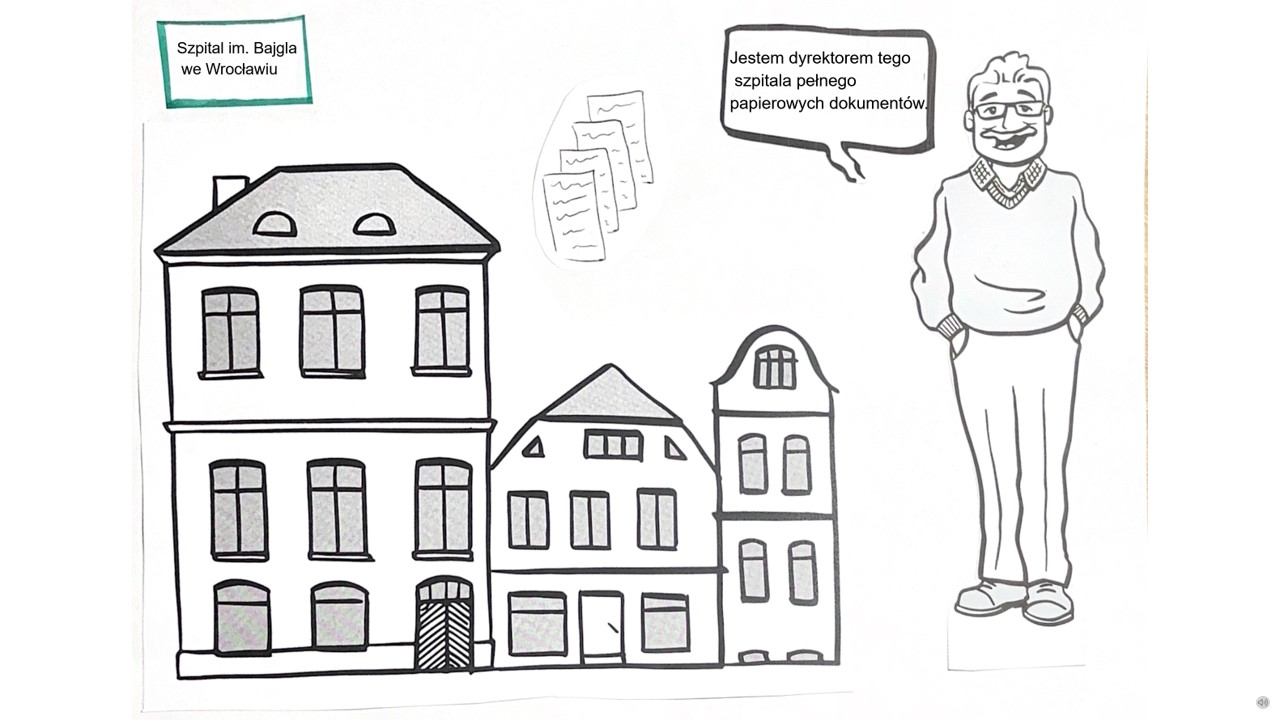
\includegraphics[width=0.8\textwidth]{Grafiki/user story/Slide1.jpg}
    \caption{User story. Slajd 1.}
    \label{fig:Slajd1}
\end{figure}

\begin{figure}[h]
    \centering
    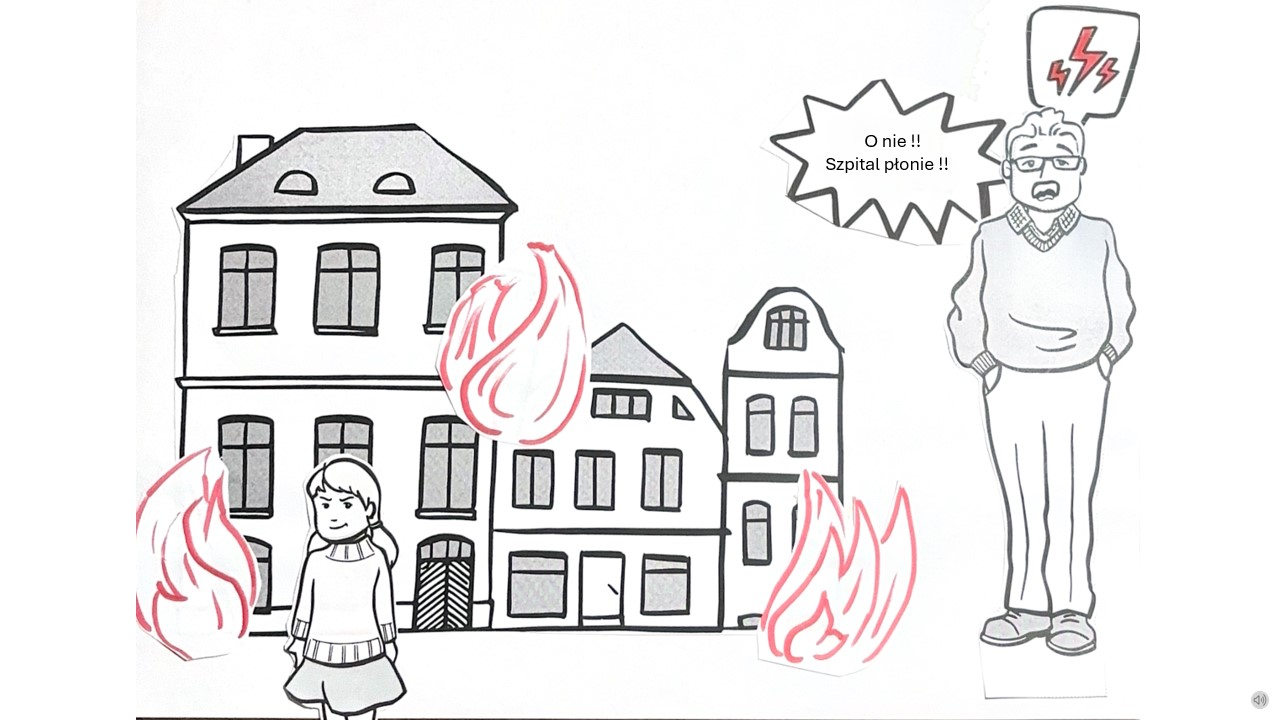
\includegraphics[width=0.8\textwidth]{Grafiki/user story/Slide2.jpg}
    \caption{User story. Slajd 2.}
    \label{fig:Slajd2}
\end{figure}

\begin{figure}[h]
    \centering
    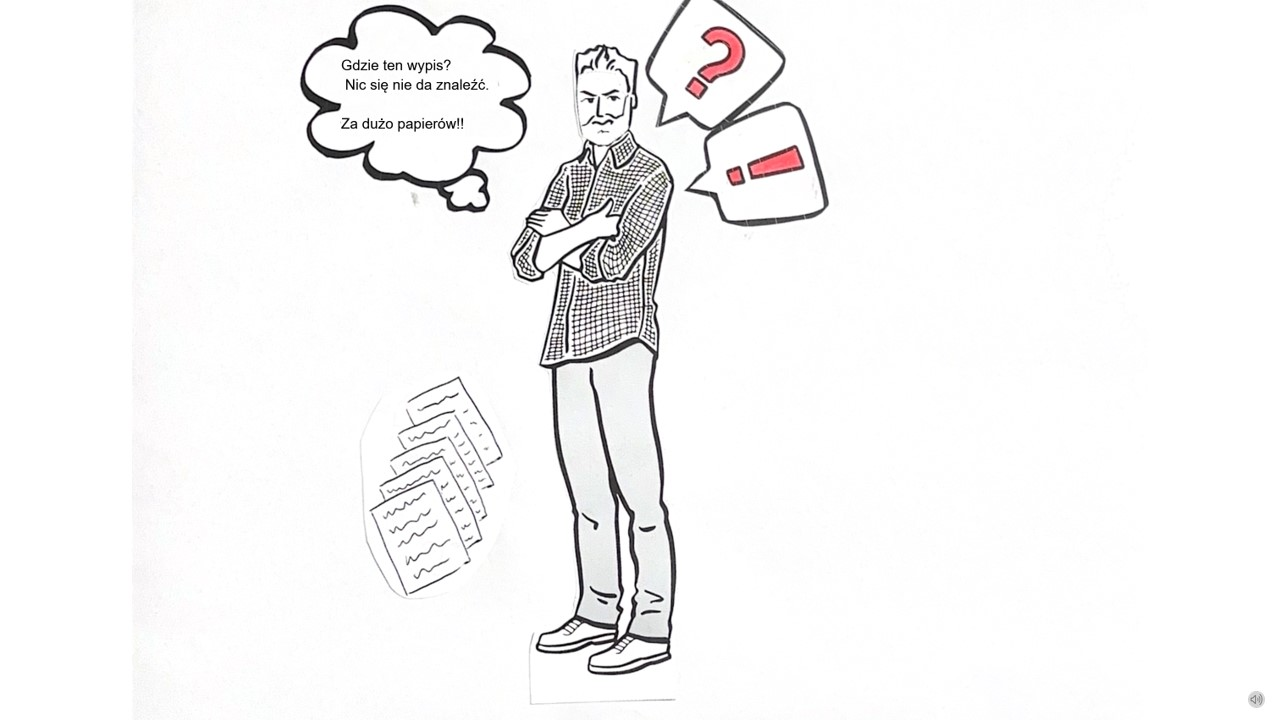
\includegraphics[width=0.8\textwidth]{Grafiki/user story/Slide3.jpg}
    \caption{User story. Slajd 3.}
    \label{fig:Slajd3}
\end{figure}

\begin{figure}[h]
    \centering
    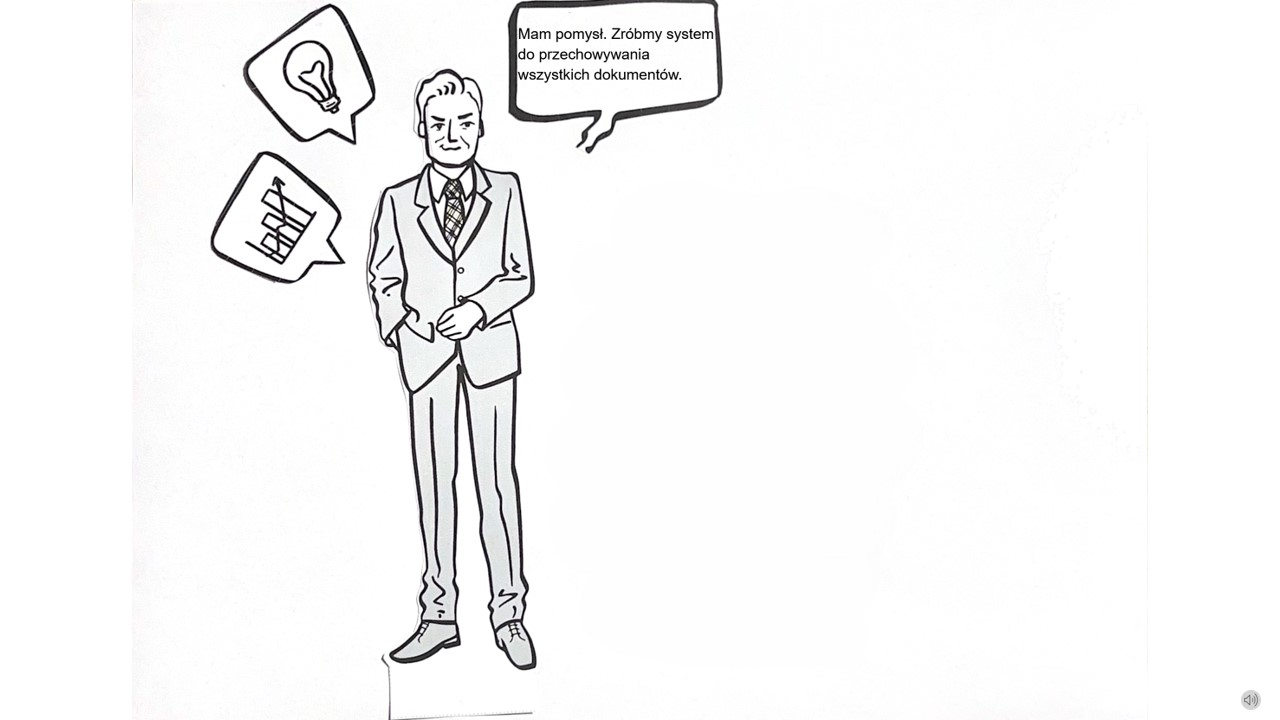
\includegraphics[width=0.8\textwidth]{Grafiki/user story/Slide4.jpg}
    \caption{User story. Slajd 4.}
    \label{fig:Slajd4}
\end{figure}

\begin{figure}[h]
    \centering
    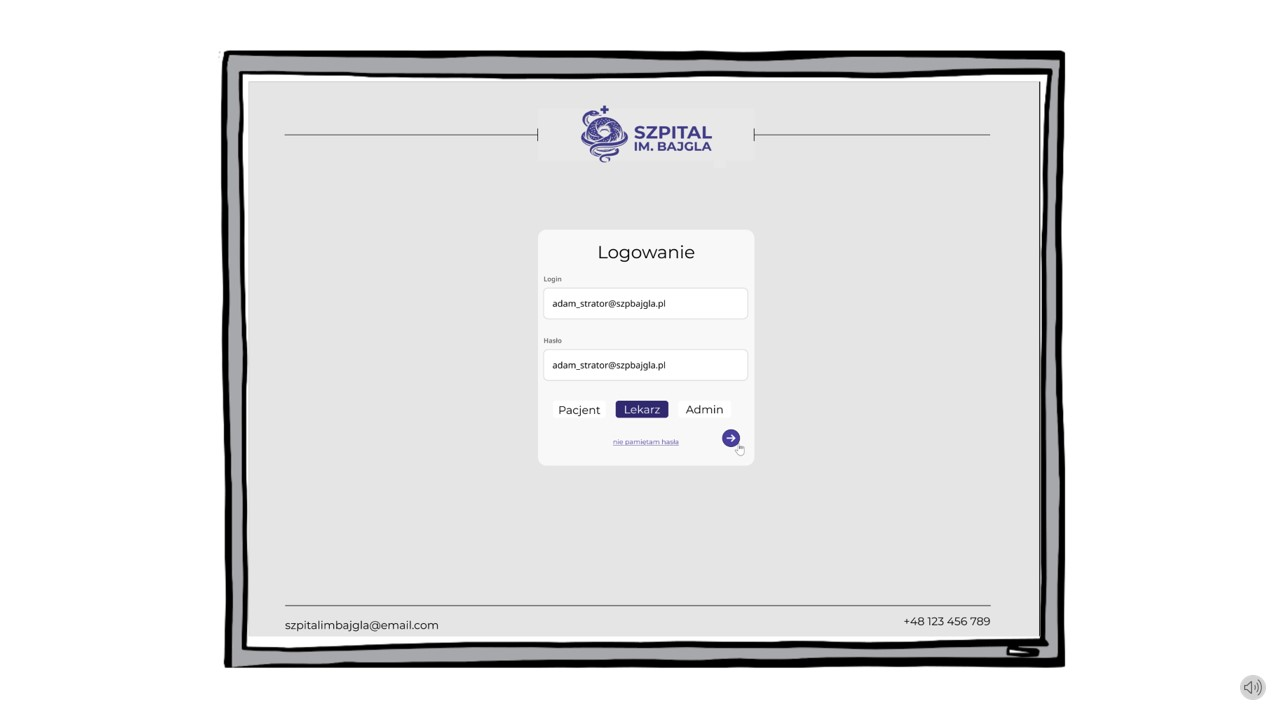
\includegraphics[width=0.8\textwidth]{Grafiki/user story/Slide5.jpg}
    \caption{User story. Slajd 5.}
    \label{fig:Slajd5}
\end{figure}

\begin{figure}[h]
    \centering
    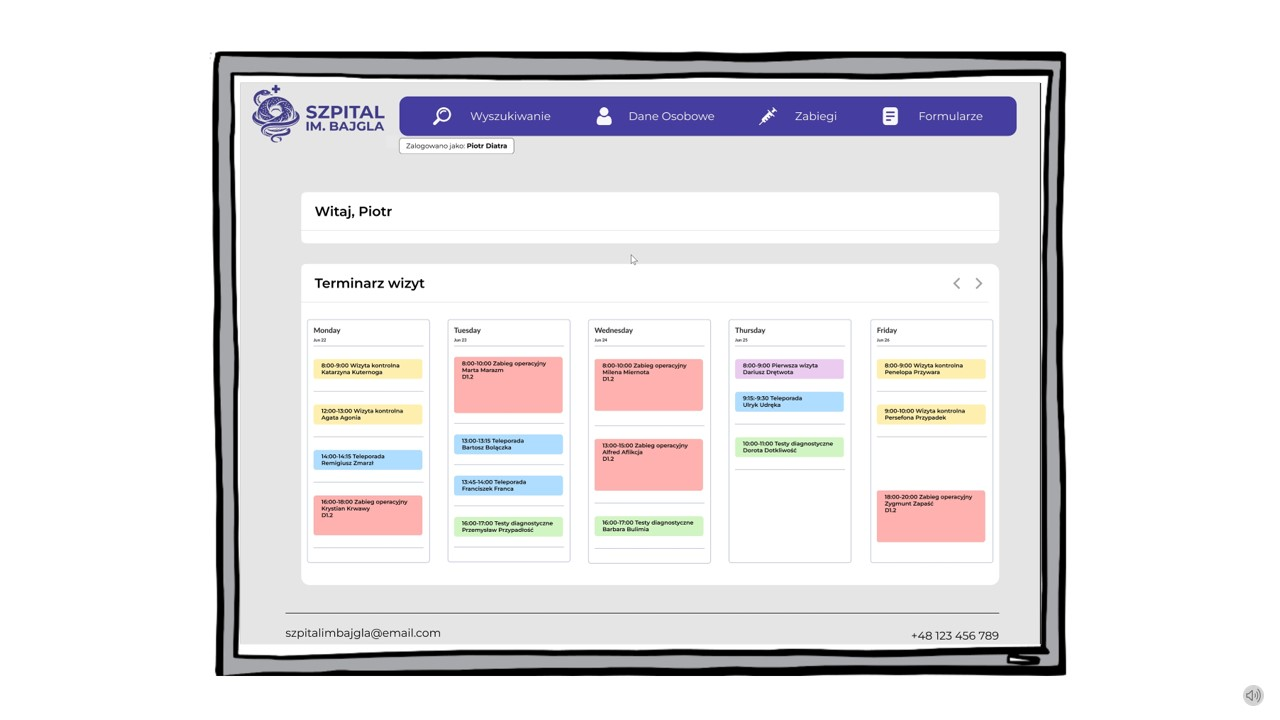
\includegraphics[width=0.8\textwidth]{Grafiki/user story/Slide6.jpg}
    \caption{User story. Slajd 6.}
    \label{fig:Slajd6}
\end{figure}

\begin{figure}[h]
    \centering
    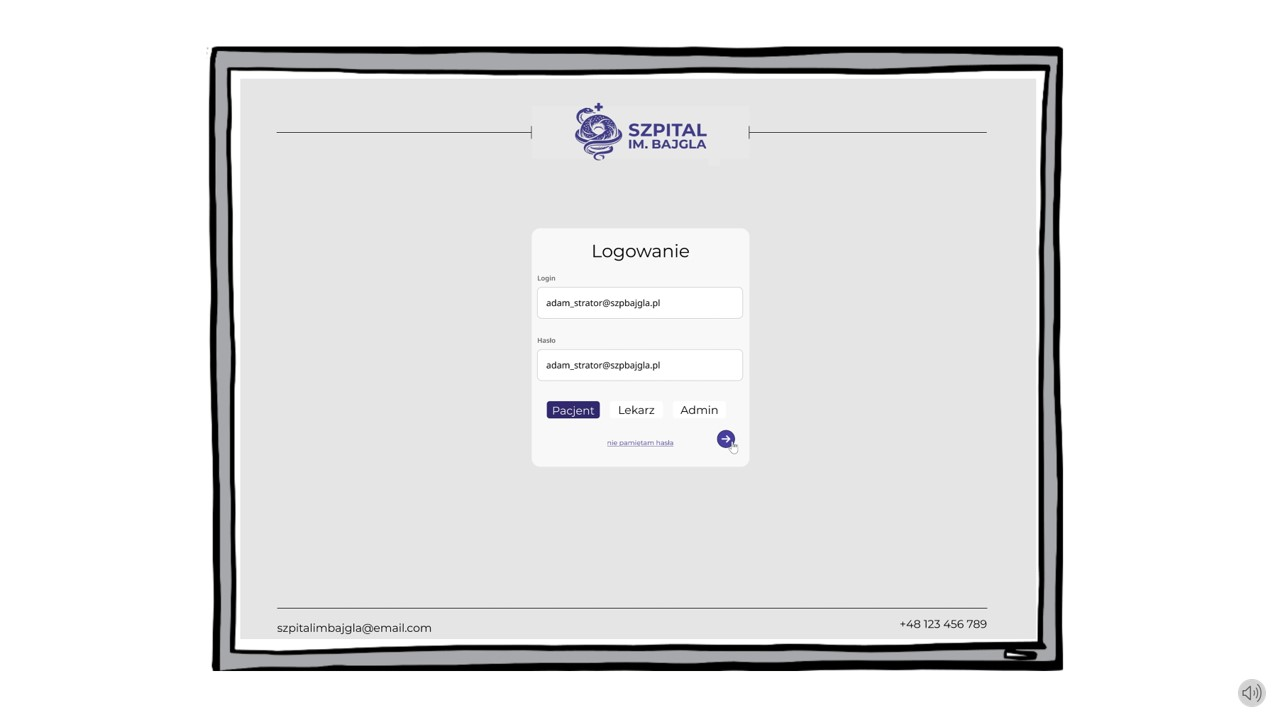
\includegraphics[width=0.8\textwidth]{Grafiki/user story/Slide7.jpg}
    \caption{User story. Slajd 7.}
    \label{fig:Slajd7}
\end{figure}

\begin{figure}[h]
    \centering
    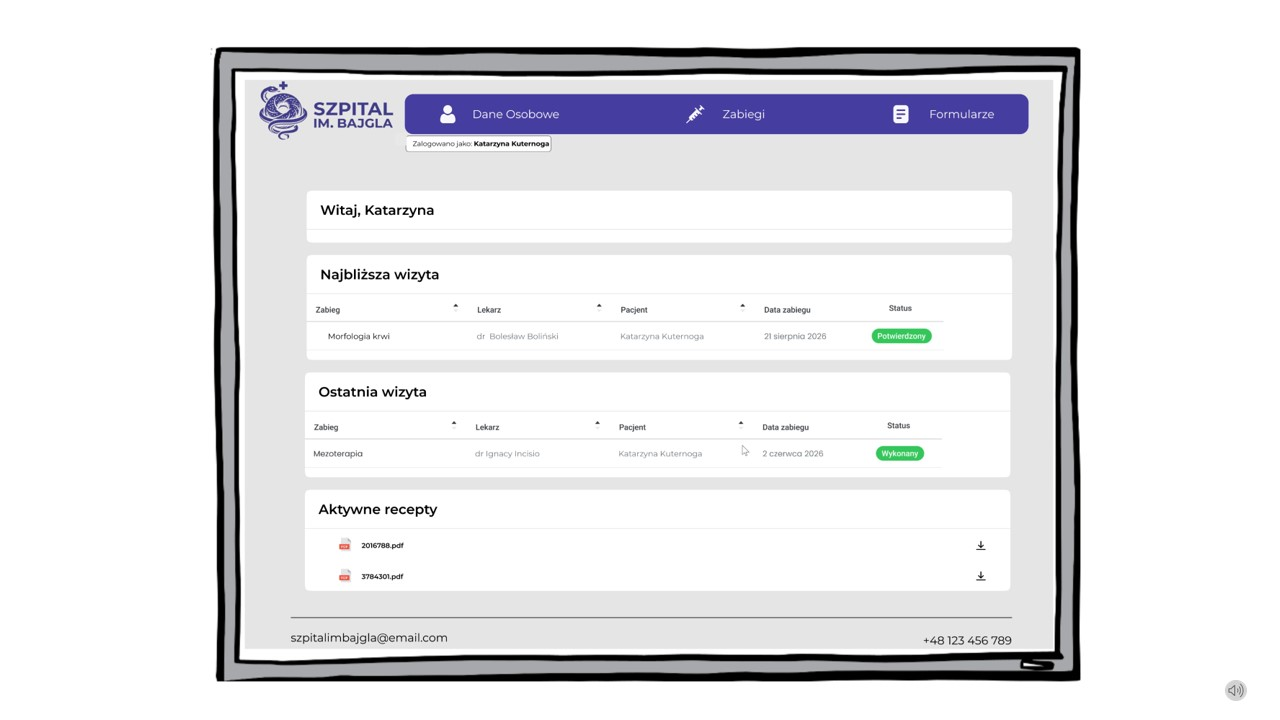
\includegraphics[width=0.8\textwidth]{Grafiki/user story/Slide8.jpg}
    \caption{User story. Slajd 8.}
    \label{fig:Slajd8}
\end{figure}

\begin{figure}[h]
    \centering
    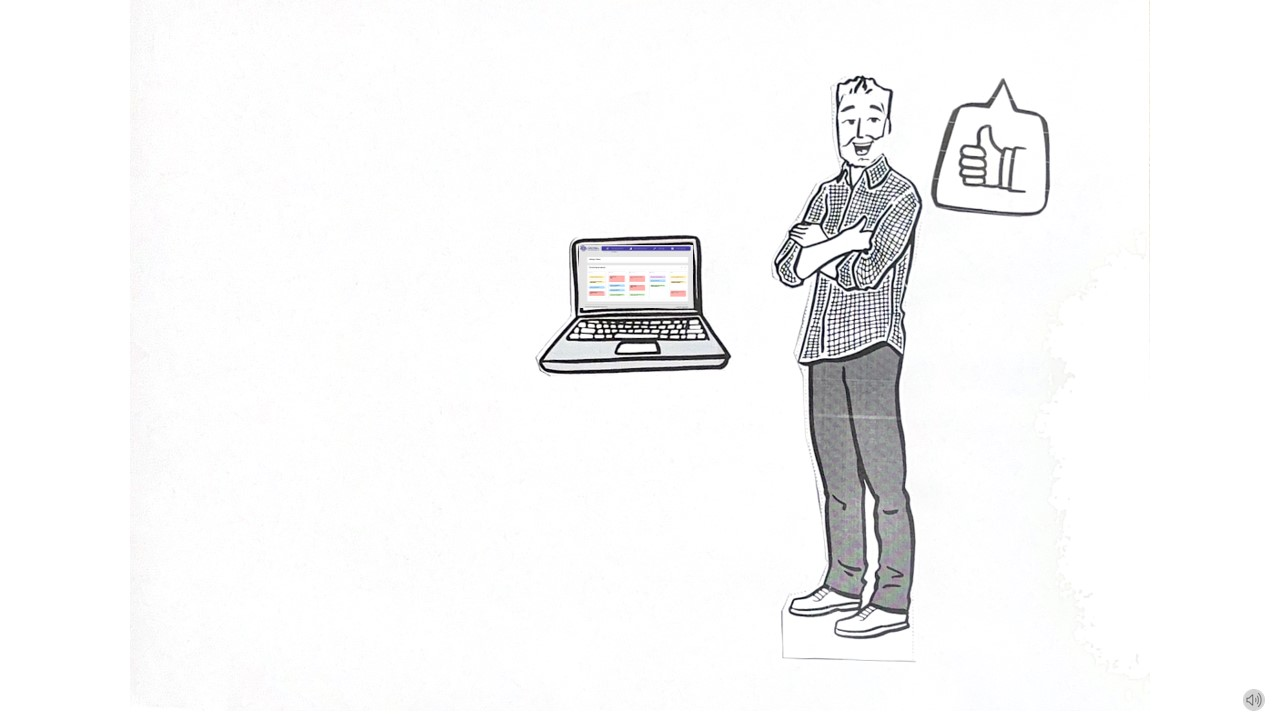
\includegraphics[width=0.8\textwidth]{Grafiki/user story/Slide9.jpg}
    \caption{User story. Slajd 9.}
    \label{fig:Slajd9}
\end{figure}


\Chapter{Propozycje rozwiązań systemu Electronic Medical Record}\label{chapter:project-idea}

\setlength{\parskip}{0pt}
\setlength{\parindent}{1.25cm}

\section{Wprowadzenie do procesu projektowego}
Na podstawie przeprowadzonej analizy funkcjonowania Szpitala im. Bajgla przygotowano kilka możliwych kierunków rozwiązania problemów związanych z organizacją dokumentacji medycznej. Ze względu na skalę placówki oraz złożoność procesów medycznych nie istnieje jedno uniwersalne rozwiązanie, które w jednakowy sposób odpowiadałoby na wszystkie potrzeby organizacyjne, techniczne i finansowe szpitala.

Proces projektowy został więc oparty na analizie różnych wariantów wdrożenia systemu EMR (Electronic Medical Record), różniących się zakresem funkcjonalności oraz poziomem zaawansowania technologicznego. Przygotowane rozwiązania uwzględniają zarówno aktualne potrzeby szpitala, jak i możliwość dalszego rozwoju systemu w przyszłości.

Istotnym aspektem procesu projektowego było również uwzględnienie potrzeb różnych grup użytkowników, w tym lekarzy, pielęgniarek, laboratoriów, administracji oraz samych pacjentów.

Przygotowane warianty obejmują trzy poziomy wdrożenia systemu: rozwiązanie podstawowe koncentrujące się na cyfryzacji najważniejszych procesów, rozwiązanie optymalne stanowiące pełny zintegrowany system EMR dla dużego szpitala oraz rozwiązanie rozszerzone obejmujące dodatkowe funkcje automatyzacji i inteligentnego zarządzania placówką.


\section{Założenia projektowe}
Każdy z analizowanych wariantów systemu został opracowany na podstawie założeń projektowych oraz wymagań związanych z funkcjonowaniem nowoczesnych systemów ochrony zdrowia. Niezależnie od zakresu wdrożenia wszystkie rozwiązania muszą zapewniać możliwość centralnego przechowywania dokumentacji medycznej oraz obsługi wielu oddziałów w ramach jednego środowiska informatycznego.

Ważnym założeniem projektowym jest również dostosowanie systemu do pracy różnych grup użytkowników. Interfejs powinien być intuicyjny oraz możliwie prosty w codziennym użytkowaniu, tak aby zmniejszyć ryzyko błędów wynikających z nieprawidłowego korzystania. Projekt zakłada także możliwość korzystania z systemu na urządzeniach stacjonarnych lub mobilnych wykorzystywanych przez personel medyczny podczas pracy na oddziałach.

Każdy z wariantów musi również spełniać wymagania dotyczące bezpieczeństwa danych medycznych oraz zgodności z regulacjami obowiązującymi na terenie Unii Europejskiej. System powinien umożliwiać kontrolę dostępu do dokumentacji, rozdzielenie uprawnień użytkowników, monitorowanie aktywności w systemie oraz zabezpieczenie danych przed utratą lub nieautoryzowanym dostępem.
\section{Wariant I – rozwiązanie podstawowe}

\subsection{Charakterystyka rozwiązania}
Wariant podstawowy zakłada cyfryzację najważniejszych procesów związanych z prowadzeniem dokumentacji medycznej w Szpitalu im. Bajgla. Rozwiązanie koncentruje się przede wszystkim na odejściu od papierowego przechowywania danych pacjentów oraz stworzeniu centralnego miejsca umożliwiającego przeglądanie podstawowej dokumentacji medycznej przez personel szpitala.
System w tej wersji ma charakter uproszczony i obejmuje wyłącznie najważniejsze funkcje niezbędne do poprawy organizacji pracy placówki. 

Projekt zakłada wykorzystanie stanowisk komputerowych znajdujących się na oddziałach bez wdrażania rozbudowanej infrastruktury mobilnej. Wariant ten został przygotowany jako rozwiązanie wymagające stosunkowo niewielkich zmian organizacyjnych oraz ograniczonego zakresu wdrożenia.

Rozwiązanie podstawowe skupia się głównie na ograniczeniu problemów związanych z przechowywaniem dokumentacji papierowej oraz uproszczeniu dostępu do informacji o pacjentach. System nie obejmuje jednak zaawansowanej automatyzacji procesów ani pełnej integracji wszystkich elementów funkcjonowania szpitala.
\subsection{Zakres funkcjonalności}
Wariant podstawowy obejmuje centralną bazę danych pacjentów umożliwiającą przechowywanie podstawowej dokumentacji medycznej w formie elektronicznej. Personel medyczny posiada możliwość przeglądania historii leczenia pacjenta, wyników badań oraz podstawowych informacji dotyczących hospitalizacji z poziomu stanowisk komputerowych znajdujących się na oddziałach.

System umożliwia również elektroniczne dodawanie wyników badań laboratoryjnych oraz dokumentacji diagnostycznej. W ramach rozwiązania przewidziano podstawowy model logowania użytkowników oraz podział uprawnień pomiędzy personelem medycznym a administracją.

Wariant obejmuje również uproszczony portal pacjenta umożliwiający dostęp do wybranych wyników badań oraz podstawowych informacji dotyczących leczenia. 

\subsection{Zalety rozwiązania}
Największą zaletą wariantu podstawowego jest stosunkowo niski poziom złożoności wdrożenia oraz ograniczone wymagania infrastrukturalne. Rozwiązanie pozwala szybko ograniczyć część problemów wynikających z dokumentacji papierowej bez konieczności przeprowadzania całkowitej reorganizacji pracy szpitala.

Wariant podstawowy może również zmniejszyć opór części personelu wobec cyfryzacji, ponieważ zakres zmian organizacyjnych pozostaje stosunkowo niewielki. System jest prostszy w utrzymaniu i wymaga mniejszej liczby szkoleń niż bardziej rozbudowane rozwiązania.

Dodatkową zaletą jest możliwość stopniowego rozwijania systemu w przyszłości poprzez dodawanie kolejnych funkcji wraz z dalszą cyfryzacją placówki.

\subsection{Ograniczenia rozwiązania}
Wariant podstawowy nie eliminuje całkowicie problemów związanych z przepływem informacji pomiędzy oddziałami oraz ograniczoną mobilnością personelu medycznego. Brak wykorzystania tabletów może powodować dalsze opóźnienia w dostępie do danych w sytuacjach wymagających szybkiej reakcji.

Ograniczeniem rozwiązania pozostaje również niski poziom automatyzacji procesów administracyjnych oraz brak zaawansowanych funkcji wspierających organizację pracy dużej placówki medycznej. System nie zapewnia pełnej integracji wszystkich procesów szpitalnych, przez co część działań nadal wymagać będzie ręcznego przekazywania informacji pomiędzy użytkownikami.

Wariant podstawowy może również okazać się rozwiązaniem niewystarczającym w perspektywie dalszego rozwoju placówki oraz rosnących wymagań związanych z cyfryzacją ochrony zdrowia.

\section{Wariant II – rozwiązanie optymalne}

\subsection{Charakterystyka rozwiązania}
Wariant optymalny zakłada wdrożenie pełnego zintegrowanego systemu EMR obejmującego wszystkie kluczowe obszary funkcjonowania szpitala. Rozwiązanie zostało zaprojektowane z myślą o dużej wielooddziałowej placówce wymagającej sprawnego przepływu informacji pomiędzy personelem medycznym, laboratoriami, diagnostyką oraz administracją.

System w tej wersji ma stanowić centralne środowisko pracy dla całego szpitala, umożliwiające bieżący dostęp do dokumentacji pacjentów w czasie rzeczywistym. Projekt zakłada wykorzystanie zarówno stanowisk komputerowych, jak i urządzeń mobilnych wykorzystywanych przez personel medyczny podczas pracy na oddziałach.

Rozwiązanie obejmuje pełną cyfryzację dokumentacji medycznej oraz automatyzację wybranych procesów organizacyjnych związanych z obiegiem informacji i wyników badań.

\subsection{Zakres funkcjonalności}
Wariant optymalny obejmuje centralną bazę danych pacjentów, elektroniczną dokumentację medyczną, elektroniczne zlecenia badań oraz bieżącą synchronizację danych pomiędzy oddziałami. Personel medyczny posiada możliwość przeglądania i aktualizowania danych pacjentów w czasie rzeczywistym z poziomu komputerów oraz tabletów.

System umożliwia automatyczne przekazywanie wyników badań laboratoryjnych i diagnostycznych do dokumentacji pacjenta oraz monitorowanie statusu wykonywanych badań. W rozwiązaniu przewidziano również moduł powiadomień informujący personel o nowych wynikach, zmianach dokumentacji lub ważnych zdarzeniach związanych z leczeniem pacjenta.

Projekt obejmuje rozbudowany system ról i poziomów dostępu, historię zmian dokumentacji, backup danych oraz mechanizmy monitorowania aktywności użytkowników. Pacjenci posiadają dostęp do portalu umożliwiającego sprawdzanie wyników badań, historii leczenia oraz wybranych informacji dotyczących hospitalizacji.


\subsection{Zalety rozwiązania}
Największą zaletą wariantu optymalnego jest pełna integracja procesów związanych z dokumentacją medyczną i przepływem informacji pomiędzy oddziałami. System znacząco usprawnia komunikację pomiędzy personelem medycznym.

Rozwiązanie poprawia organizację pracy szpitala poprzez umożliwienie szybkiego dostępu do aktualnych danych pacjentów. Wykorzystanie urządzeń mobilnych zwiększa wygodę pracy personelu i umożliwia dostęp do dokumentacji bez konieczności powrotu do stacjonarnych stanowisk komputerowych.

Wariant optymalny zapewnia również wysoki poziom bezpieczeństwa danych medycznych oraz możliwość dalszej rozbudowy systemu w przyszłości. Rozwiązanie odpowiada potrzebom dużej placówki medycznej i pozostaje zgodne z kierunkiem rozwoju nowoczesnych systemów eHealth w Unii Europejskiej.

\subsection{Ograniczenia rozwiązania}
Wdrożenie wariantu optymalnego wymaga większych nakładów organizacyjnych oraz technicznych niż rozwiązanie podstawowe. Konieczne staje się przygotowanie odpowiedniej infrastruktury sieciowej, zakup urządzeń mobilnych oraz przeprowadzenie szkoleń dla personelu medycznego.

Rozwiązanie wiąże się również z większym poziomem zmian organizacyjnych w codziennym funkcjonowaniu placówki. Część pracowników może początkowo odczuwać trudności związane z przejściem na w pełni cyfrowy model pracy.

Wariant wymaga także bardziej rozbudowanego wsparcia technicznego oraz regularnego utrzymania systemu ze względu na większą liczbę funkcjonalności i użytkowników.

\section{Wariant III – rozwiązanie rozszerzone}

\subsection{Charakterystyka rozwiązania}
Wariant rozszerzony zakłada rozbudowę systemu EMR o dodatkowe funkcje analizy danych oraz częściowej automatyzacji organizacji pracy szpitala. W przeciwieństwie do wariantu optymalnego rozwiązanie nie skupia się wyłącznie na elektronicznej dokumentacji i komunikacji pomiędzy oddziałami, ale dodatkowo umożliwia bieżące monitorowanie działania placówki oraz analizowanie danych organizacyjnych.

System ma wspierać dyrekcję i administrację w kontrolowaniu funkcjonowania szpitala poprzez wykorzystanie bardziej zaawansowanych narzędzi raportowania, monitorowania i analizy danych generowanych podczas codziennej pracy placówki.
\subsection{Zakres funkcjonalności}
Wariant rozszerzony obejmuje dodatkowe moduły analityczne oraz funkcje automatyzacji procesów organizacyjnych. System może automatycznie tworzyć raporty dotyczące obciążenia oddziałów, liczby pacjentów, czasu oczekiwania na badania lub wykorzystania personelu medycznego.

Rozwiązanie może również generować inteligentne powiadomienia dotyczące problemów organizacyjnych, takich jak opóźnienia badań, przeciążenie oddziałów lub brakujące elementy dokumentacji. Dodatkowo przewidziano możliwość integracji z wybranymi urządzeniami medycznymi, dzięki czemu część danych mogłaby trafiać do systemu automatycznie bez konieczności ręcznego przepisywania wyników.

W projekcie uwzględniono także bardziej rozbudowaną aplikację pacjenta umożliwiającą szerszy kontakt ze szpitalem oraz dostęp do większej liczby informacji dotyczących leczenia.
\subsection{Zalety rozwiązania}
Największą zaletą wariantu rozszerzonego jest możliwość wykorzystania danych do wspomagania organizacji pracy szpitala oraz szybszego wykrywania problemów związanych z funkcjonowaniem placówki. System może ułatwić analizowanie obciążenia oddziałów oraz usprawnić zarządzanie personelem i zasobami szpitala.

Dodatkową zaletą jest możliwość dalszej rozbudowy systemu o kolejne funkcje automatyzacji oraz integracji z dodatkowymi urządzeniami i modułami w przyszłości.
\subsection{Ograniczenia rozwiązania}
Wariant rozszerzony wymaga bardziej rozbudowanej infrastruktury technicznej oraz większego wsparcia administracyjnego niż wariant optymalny. Rozwiązanie wiąże się również z większym poziomem skomplikowania utrzymania systemu oraz koniecznością bardziej zaawansowanego zarządzania jego działaniem.

Dodatkowo w przypadku integracji mechanizmów analizy danych opartych na sztucznej inteligencji zaistniałaby konieczność dostosowania systemu do wymagań wynikających z regulacji AI Act oraz przepisów dotyczących ochrony danych osobowych. Oznaczałoby to między innymi konieczność odpowiedniego dokumentowania sposobu działania systemu, monitorowania wykorzystania modeli AI oraz zapewnienia przejrzystości procesu przetwarzania danych medycznych.

Konieczne byłoby również informowanie pacjentów oraz pracowników o wykorzystaniu mechanizmów sztucznej inteligencji w analizie danych medycznych i organizacyjnych. W zależności od zakresu działania systemu mogłoby być wymagane także wdrożenie dodatkowych procedur związanych z nadzorem nad działaniem modeli AI oraz bezpieczeństwem danych.

\section{Porównanie wariantów}

\subsection{Tabela porównawcza}

\renewcommand{\arraystretch}{1.3}

\begin{longtable}{|p{4cm}|p{3cm}|p{3cm}|p{3cm}|}

\caption{Porównanie wariantów systemu EMR}
\label{tab:warianty_emr} \\

\hline
\textbf{Kryterium} &
\shortstack{\textbf{Wariant I} \\ podstawowy} &
\shortstack{\textbf{Wariant II} \\ optymalny} &
\shortstack{\textbf{Wariant III} \\ rozszerzony} \\
\hline
\endfirsthead

\hline
\textbf{Kryterium} &
\shortstack{\textbf{Wariant I} \\ podstawowy} &
\shortstack{\textbf{Wariant II} \\ optymalny} &
\shortstack{\textbf{Wariant III} \\ rozszerzony} \\
\hline
\endhead

Zakres cyfryzacji dokumentacji &
częściowy &
pełny &
pełny \\
\hline

Centralna baza danych pacjentów &
tak &
tak &
tak \\
\hline

Elektroniczna dokumentacja medyczna &
podstawowa &
pełna &
pełna \\
\hline

Integracja oddziałów &
ograniczona &
pełna &
pełna \\
\hline

Dostęp do danych w czasie rzeczywistym &
częściowy &
tak &
tak \\
\hline

Mobilny dostęp dla personelu &
brak &
tablety i urządzenia mobilne &
tablety i urządzenia mobilne \\
\hline

Portal pacjenta &
podstawowy &
rozbudowany &
rozbudowany \\
\hline

Automatyczne przekazywanie wyników badań &
częściowe &
tak &
tak \\
\hline

Moduły analityczne i raportowanie &
brak &
podstawowe raporty &
zaawansowana analiza danych \\
\hline

Analiza obciążenia oddziałów &
brak &
brak &
rozbudowana \\
\hline

Inteligentne powiadomienia i alerty &
brak &
podstawowe &
rozbudowane \\
\hline

Integracja z urządzeniami medycznymi &
brak &
ograniczona &
rozszerzona \\
\hline

Wsparcie organizacji pracy szpitala &
podstawowe &
wysokie &
bardzo wysokie \\
\hline

Bezpieczeństwo danych i kontrola dostępu &
podstawowe &
wysokie &
bardzo wysokie \\
\hline

Wykorzystanie analizy danych AI &
brak &
brak &
tak \\
\hline

Wymagania związane z AI Act &
nie dotyczy &
nie dotyczy &
wymagane \\
\hline

Poziom automatyzacji &
niski &
średni &
wysoki \\
\hline

Stopień skomplikowania wdrożenia &
niski &
wysoki &
bardzo wysoki \\
\hline

Wymagania infrastrukturalne &
niskie &
średnie &
wysokie \\
\hline

Zakres szkoleń personelu &
niewielki &
duży &
bardzo duży \\
\hline

\end{longtable}

\subsection{Analiza porównawcza}

Przeprowadzona analiza pokazuje, że każdy z wariantów odpowiada na potrzeby szpitala w innym stopniu. Wariant podstawowy umożliwia częściową cyfryzację dokumentacji oraz ograniczenie ilości dokumentów papierowych, jednak nie zapewnia pełnej integracji procesów medycznych i administracyjnych. Rozwiązanie to charakteryzuje się najniższymi kosztami wdrożenia i najmniejszym poziomem skomplikowania infrastruktury.

Wariant optymalny zapewnia pełną cyfryzację dokumentacji medycznej, integrację oddziałów oraz sprawny dostęp do danych pacjentów w czasie rzeczywistym. Rozwiązanie oferuje szeroki zakres funkcjonalności przy jednoczesnym zachowaniu umiarkowanych wymagań organizacyjnych i infrastrukturalnych.

Wariant rozszerzony oferuje najwyższy poziom automatyzacji oraz dodatkowe funkcje związane z analizą danych i integracją elementów sztucznej inteligencji. Rozwiązanie wiąże się jednak z największym poziomem złożoności wdrożenia, wysokimi kosztami utrzymania oraz dodatkowymi wymaganiami prawnymi związanymi między innymi z AI Act.

\section{Wybór rozwiązania docelowego}

Na podstawie przeprowadzonej analizy jako rozwiązanie docelowe wybrano wariant optymalny. Rozwiązanie to stanowi kompromis pomiędzy zakresem funkcjonalności, kosztami wdrożenia oraz możliwościami organizacyjnymi szpitala.

Wybrany wariant spełnia wszystkie kluczowe wymagania placówki związane z pełną cyfryzacją dokumentacji medycznej, poprawą przepływu informacji oraz zwiększeniem dostępności danych pacjentów. Jednocześnie nie wymaga tak rozbudowanej infrastruktury oraz tak dużych zmian organizacyjnych jak wariant rozszerzony.

Klient zdecydował się na rozwiązanie, które jest możliwe do wdrożenia w obecnych warunkach finansowych szpitala, a jednocześnie zapewnia możliwość dalszej rozbudowy systemu w przyszłości.
\section{Kryteria oceny rozwiązania}
Po wprowadzeniu docelowego wariantu systemu EMR zostanie przeprowadzona ocena skuteczności wdrożonego rozwiązania na podstawie określonych kryteriów funkcjonalnych, organizacyjnych oraz technicznych. Celem oceny będzie sprawdzenie, w jakim stopniu system usprawni funkcjonowanie szpitala oraz ograniczy problemy związane z papierowym obiegiem dokumentacji.

Pierwszym kryterium będzie poziom cyfryzacji dokumentacji medycznej. Zostanie on określony jako procent dokumentów obsługiwanych elektronicznie w stosunku do całej dokumentacji powstającej w codziennej pracy szpitala. Pod uwagę zostaną wzięte między innymi karty pacjentów, wyniki badań, zlecenia lekarskie, raporty pielęgniarskie, wypisy oraz dokumenty administracyjne. Im większy udział dokumentów obsługiwanych w systemie cyfrowym, tym wyższy będzie poziom cyfryzacji placówki.

Drugim kryterium będzie czas dostępu do dokumentacji pacjenta. Pomiar zostanie wykonany poprzez sprawdzenie, ile czasu potrzebuje uprawniony użytkownik na odnalezienie historii leczenia, aktualnych wyników badań lub ostatnich zleceń lekarskich. Analiza będzie obejmowała typowe sytuacje pracy szpitala, takie jak przyjęcie pacjenta, obchód lekarski lub przygotowanie wypisu.

Trzecim kryterium będzie dostępność systemu dla użytkowników w codziennej pracy. Ocenie zostanie poddana liczba stanowisk oraz urządzeń umożliwiających korzystanie z systemu, możliwość pracy mobilnej oraz dostępność danych na oddziałach, na których personel nie pracuje stale przy komputerze. Szczególnie istotne będzie sprawdzenie, czy lekarz lub pielęgniarka będą mogli uzyskać dostęp do danych pacjenta bez konieczności opuszczania oddziału lub przerywania wykonywanych czynności.

Czwartym kryterium będzie bezpieczeństwo i kontrola dostępu do danych. W ramach oceny sprawdzone zostanie, czy system posiada role użytkowników, indywidualne konta, historię zmian dokumentacji, rejestr logowań oraz możliwość ograniczania dostępu do danych zgodnie z zakresem obowiązków pracownika. Kryterium to będzie mierzone między innymi liczbą dostępnych poziomów uprawnień oraz możliwością monitorowania aktywności użytkowników w systemie.

\Chapter{Założenia organizacyjne wdrożenia systemu EMR}
\label{chapter:implementation}

\section{Wprowadzenie}

Wdrożenie systemu EMR w Szpitalu im. Bajgla stanowi nie tylko projekt technologiczny, ale również dużą zmianę organizacyjną obejmującą sposób codziennej pracy personelu medycznego i administracyjnego. Oprócz przygotowania samego systemu konieczne jest również zaplanowanie sposobu wdrożenia rozwiązania, migracji dokumentacji oraz organizacji pracy użytkowników w okresie przejściowym.

Celem przedstawionych założeń jest ograniczenie problemów organizacyjnych i technicznych związanych z cyfryzacją placówki przy jednoczesnym zachowaniu ciągłości pracy szpitala. Założenia te mają również zmniejszyć ryzyko błędów podczas wdrożenia oraz ułatwić adaptację personelu do nowego środowiska pracy.

\section{Etapowe wdrażanie systemu}

Ze względu na skalę działalności Szpitala im. Bajgla wdrożenie systemu powinno odbywać się etapowo. Rozwiązanie to pozwala ograniczyć ryzyko organizacyjne oraz uniknąć sytuacji, w której jednoczesna zmiana sposobu pracy całej placówki mogłaby doprowadzić do problemów z funkcjonowaniem oddziałów.

W pierwszym etapie system powinien zostać wdrożony na wybranych oddziałach o mniejszym stopniu złożoności organizacyjnej. Pozwoli to przetestować działanie podstawowych funkcjonalności oraz wprowadzić ewentualne poprawki przed rozszerzeniem systemu na pozostałe jednostki szpitala. Dopiero po zakończeniu fazy pilotażowej rozwiązanie mogłoby zostać wdrożone na oddziałach wymagających szybkiego przepływu informacji, takich jak SOR lub oddział intensywnej terapii.

Migracja dokumentacji papierowej również powinna odbywać się stopniowo. W pierwszej kolejności do systemu przenoszone byłyby aktualne dane pacjentów oraz dokumentacja wykorzystywana w bieżącej pracy oddziałów. Archiwalna dokumentacja mogłaby być cyfryzowana etapowo w późniejszym okresie, co pozwoliłoby ograniczyć koszty i obciążenie organizacyjne związane z jednoczesnym przetwarzaniem bardzo dużej ilości danych.

W okresie przejściowym przewidziano równoczesne funkcjonowanie części dokumentacji papierowej i cyfrowej. Takie rozwiązanie umożliwia stopniowe przyzwyczajanie personelu do nowego systemu oraz ogranicza ryzyko utraty dostępu do danych podczas początkowego etapu wdrożenia.

\section{Szkolenie i organizacja pracy personelu}

Wdrożenie nowego systemu wymaga odpowiedniego przygotowania personelu medycznego oraz administracyjnego do pracy w środowisku cyfrowym. Z tego powodu przed rozpoczęciem korzystania z systemu konieczne jest przeprowadzenie szkoleń obejmujących podstawowe funkcjonalności oraz procedury pracy z dokumentacją elektroniczną.

Szkolenia powinny być dostosowane do zakresu obowiązków poszczególnych grup użytkowników. Lekarze, pielęgniarki, laboranci oraz pracownicy administracyjni korzystają z różnych elementów systemu, dlatego zakres przekazywanych informacji powinien odpowiadać rzeczywistym potrzebom danej grupy.

W celu ograniczenia problemów organizacyjnych przewidziano również przygotowanie podstawowych procedur korzystania z systemu. Dotyczy to między innymi sposobu dodawania dokumentacji, aktualizowania danych pacjentów, przekazywania informacji pomiędzy oddziałami oraz postępowania w sytuacjach awaryjnych.

Istotnym elementem organizacji pracy jest również określenie odpowiedzialności za wprowadzanie i aktualizowanie danych. Każdy użytkownik powinien posiadać indywidualne konto umożliwiające identyfikację działań wykonywanych w systemie. Rozwiązanie to pozwala ograniczyć ryzyko błędów oraz zwiększa bezpieczeństwo dokumentacji medycznej.

\section{Założenia techniczne i bezpieczeństwo systemu}

Projektowany system zakłada wykorzystanie centralnej bazy danych umożliwiającej przechowywanie dokumentacji pacjentów w jednym spójnym środowisku. Dzięki temu możliwa będzie synchronizacja danych pomiędzy oddziałami oraz dostęp do aktualnych informacji w czasie rzeczywistym.

Istotnym założeniem projektu jest zapewnienie odpowiedniego poziomu bezpieczeństwa danych medycznych. System powinien wykorzystywać indywidualne konta użytkowników, podział poziomów dostępu oraz szyfrowanie danych i transmisji informacji. Dzięki temu możliwe będzie ograniczenie dostępu do dokumentacji wyłącznie do osób posiadających odpowiednie uprawnienia.

W projekcie przewidziano także tworzenie regularnych kopii zapasowych oraz procedur odzyskiwania danych po awarii systemu. Rozwiązanie to ma ograniczyć ryzyko utraty dokumentacji medycznej oraz umożliwić szybkie przywrócenie działania systemu w przypadku problemów technicznych.

Dodatkowo system powinien umożliwiać monitorowanie aktywności użytkowników oraz rejestrowanie zmian wykonywanych w dokumentacji medycznej. Funkcjonalność ta jest istotna zarówno z perspektywy bezpieczeństwa danych, jak i zgodności z wymaganiami dotyczącymi ochrony informacji medycznych obowiązującymi w Unii Europejskiej.

\section{Postępowanie w sytuacjach awaryjnych}

Ze względu na całodobowy charakter pracy szpitala konieczne jest przygotowanie procedur umożliwiających funkcjonowanie placówki również w przypadku czasowej niedostępności systemu. W sytuacji awarii personel powinien posiadać możliwość przejścia na uproszczony tryb pracy oraz czasowego wykorzystania dokumentacji zastępczej do momentu przywrócenia pełnej funkcjonalności systemu.

W projekcie przewidziano również stałe wsparcie techniczne po wdrożeniu systemu. W początkowym okresie działania rozwiązania szczególnie ważne będzie szybkie reagowanie na problemy zgłaszane przez użytkowników oraz możliwość bieżącego wprowadzania poprawek organizacyjnych i technicznych.
\chapter{Kosztorys wdrożenia systemu EMR}
\label{chapter:costs}

\section{Wprowadzenie i metodyka}

Niniejszy rozdział przedstawia szczegółowy kosztorys wdrożenia systemu Electronic Medical Record (EMR) w Szpitalu im. Bajgla we Wrocławiu. Kosztorys obejmuje nakłady inwestycyjne (CAPEX), koszty operacyjne (OPEX) oraz całkowity koszt posiadania (TCO) w horyzoncie 5 lat. Wszystkie trzy warianty rozwiązania opisane w rozdziale~\ref{chapter:project-idea} wyceniono na tym samym poziomie szczegółowości, co zapewnia pełną porównywalność, a wycenę szczegółową rozwinięto dla rekomendowanego Wariantu~II, wybranego przez klienta jako wdrażane rozwiązanie.

\subsection{Zastosowane zasady}

\begin{itemize}
    \item \textbf{Estymacja oddolna (bottom-up)} – każdy koszt wynika z konkretnej pozycji (osobo-miesiąc, sztuka sprzętu, jednostka zasobu chmurowego).
    \item \textbf{Rozdział CAPEX/OPEX} oraz pełny koszt posiadania (TCO) w horyzoncie 5 lat.
    \item \textbf{Oddzielenie kosztu wytworzenia od ceny kontraktowej} – jawny narzut realizacyjny oraz marża wykonawcy, prowadzące do ceny kontraktowej.
    \item \textbf{Scenariusze i analiza wrażliwości} – wartości punktowe uzupełniono o wariant optymistyczny, bazowy i pesymistyczny oraz macierz ryzyk kosztowych.
    \item \textbf{Benchmarki rynkowe} – stawki pracy i koszty jednostkowe odniesione do publikowanych źródeł.
\end{itemize}

\subsection{Podstawa cenowa}

Kwoty podano w PLN, w wartościach \textbf{netto} (poziom cen 2026). Stawki pracy w kategorii~A ujęto w kwocie netto na umowie B2B -- VAT od faktur podwykonawców podlega odliczeniu u wykonawcy (por. sekcję~\ref{sec:capex_ii}). VAT 23\% dotyczy wyłącznie \textbf{ceny kontraktowej} płatnej przez szpital (tab.~\ref{tab:komercyjny}). Benchmarki stawek: \cite{Hays_2026, NoFluffJobs_2025}; koszty chmury: \cite{Azure_Pricing_2026}.

\section{Założenia wejściowe}

\subsection{Profil placówki, populacja i dane}

Aby oprzeć kosztorys na realnej skali dużego szpitala klinicznego, założenia oparto na podstawie danych Uniwersyteckiego Szpitala Klinicznego we Wrocławiu z raportu rocznego za rok 2014 \cite{USK_Raport_2014}. Część parametrów (liczba oddziałów, zatrudnienie, liczba przyjęć i porad) pochodzi bezpośrednio z raportu; pozostałe -- nieujęte w raporcie, lecz niezbędne do wymiarowania systemu (liczba łóżek, konta i obciążenie systemu, wolumeny danych) oszacowano. Pochodzenie każdego parametru oznaczono w kolumnie „Źródło”.

\begin{table}[h]
\centering
\small
\renewcommand{\arraystretch}{1.15}
\begin{tabular}{|L{5.4cm}|L{6.4cm}|L{2.4cm}|}
\hline
\rowcolor{gray!20}\textbf{Parametr} & \textbf{Wartość} & \textbf{Źródło} \\
\hline
Liczba oddziałów / klinik & 37 oddziałów / 23 kliniki & raport \\
\hline
Poradnie / pracownie diagnostyczne & 37 / 31 & raport \\
\hline
Zatrudnienie ogółem & 2 897 (w tym 2 170 umów o pracę, 89 kontraktów) & raport \\
\hline
Konta personelu w systemie EMR & 2 600 & szacunek \\
\hline
Liczba łóżek & 1 150 & szacunek \\
\hline
Przyjęcia w szpitalu ogółem rocznie & 116 423 & raport \\
\hline
\quad w tym oddziały / SOR / dializy & 58 167 / 34 539 / 23 717 & raport \\
\hline
Porady ambulatoryjne rocznie & 110 227 & raport \\
\hline
Aktywne konta pacjentów (portal) & 400 000 & szacunek \\
\hline
Szczytowa liczba użytkowników jednoczesnych & 700 & szacunek \\
\hline
Szczytowe obciążenie API & 1 200 zap./s & szacunek \\
\hline
Przyrost danych ustrukturyzowanych / dokumentów rocznie & 300 GB / 2 TB & szacunek \\
\hline
Dane obrazowe (PACS/DICOM) rocznie & 50 TB & szacunek \\
\hline
Wymagany okres retencji dokumentacji medycznej & 20 lat & wymóg prawny \\
\hline
Tryb pracy & 24/7/365 & raport \\
\hline
\end{tabular}
\caption{Założenia wejściowe -- na podstawie USK Wrocław (raport 2014)}
\label{tab:zalozenia}
\end{table}

\paragraph{Uwagi do szacunków.} Liczbę łóżek (ok.~1 150) oszacowano z liczby przyjęć na oddziały (58 167) przy średnim czasie hospitalizacji ok.~5,5 dnia i obłożeniu ok.~72\%. Liczbę kont personelu EMR (ok.~2 600) przyjęto jako personel medyczny i administracyjny z dostępu do systemu (z pominięciem wolontariatu i części umów zlecenie). Wolumeny danych oraz obciążenie systemu oszacowano proporcjonalnie do skali aktywności placówki. Dane skali pochodzą z USK Wrocław (raport 2014) jako benchmark dużego szpitala klinicznego; dla mniejszej placówki wymiarowanie należy skorygować proporcjonalnie.

\subsection{Założenia dotyczące floty sprzętu}

Aby przedstawić założenia dotyczące modelu sprzętowego w sposób rzetelny, przyjęto następujące założenia eksploatacyjne, uwzględnione w kosztach inwestycyjnych i operacyjnych:

\begin{itemize}
    \item \textbf{Bufor sprzętowy} – pula zapasowa na poziomie 12\% liczby urządzeń mobilnych i stanowisk (sprzęt zastępczy na czas serwisu).
    \item \textbf{Cykl wymiany} – tablety 4 lata, stanowiska komputerowe 5 lat, infrastruktura sieciowa 6--7 lat.
    \item \textbf{Ubytki i uszkodzenia} – zakładana stopa utraty/uszkodzeń tabletów 5\% rocznie.
    \item \textbf{Finansowanie odtworzeniowe} – koszty bufora, wymiany i ubytków pokrywane są z rezerwy odtworzeniowej w OPEX (tab.~\ref{tab:opex_suma}) oraz w scenariuszu pesymistycznym kosztorysu.
\end{itemize}

\section{Benchmarki rynkowe i źródła danych}

W celu uniknięcia stawek „bez źródła” przyjęte założenia kosztowe odniesiono do publikowanych benchmarków rynkowych oraz analiz wdrożeń systemów EMR/EHR w szpitalach o porównywalnej skali.

\begin{table}[h]
\centering
\small
\renewcommand{\arraystretch}{1.2}
\begin{tabular}{|p{4.2cm}|p{5.8cm}|p{3.2cm}|}
\hline
\rowcolor{gray!20}\textbf{Obszar} & \textbf{Źródło} & \textbf{Zastosowanie} \\
\hline
Stawki B2B specjalistów IT & Hays Salary Guide \cite{Hays_2026}, NoFluffJobs \cite{NoFluffJobs_2025} & Kategoria A \\
\hline
Cennik chmury (IaaS/PaaS) & Microsoft Azure Pricing \cite{Azure_Pricing_2026} & Kategoria B, OPEX \\
\hline
Wymagania integracji krajowej & Centrum e-Zdrowia \cite{CeZ_P1_2025} & Kategoria F \\
\hline
Benchmarki wdrożeń EMR/EHR & Software Finder (Oracle Cerner) \cite{SoftwareFinder_Cerner_2026}, The Pricer (Epic EMR) \cite{ThePricer_Epic_2024} & Walidacja CAPEX/TCO \\
\hline
\end{tabular}
\caption{Źródła benchmarków przyjętych w kosztorysie}
\label{tab:benchmarki}
\end{table}

Oprócz benchmarków jednostkowych przeprowadzono również walidację całkowitego budżetu projektu względem publicznie opisywanych wdrożeń systemów EMR/EHR realizowanych w szpitalach o porównywalnej skali działalności.

Według zestawienia Software Finder dla systemu Oracle Cerner \cite{SoftwareFinder_Cerner_2026}, koszty wdrożenia w szpitalach posiadających około 500 łóżek wynoszą zazwyczaj od 12 do 30 mln USD, przy rocznych kosztach utrzymania na poziomie 1,5–3 mln USD. Odpowiada to przedziałowi około 48–120 mln PLN (przy kursie 1 USD = 4,0 PLN).

Analizy dotyczące systemu Epic EMR wskazują natomiast, że wdrożenia w dużych organizacjach (zakładając 1000 łóżek) mogą osiągać poziom 50–100 mln USD, co odpowiada około 200–400 mln PLN \cite{ThePricer_Epic_2024}.

\begin{table}[h]
\centering
\small
\renewcommand{\arraystretch}{1.2}
\setlength{\tabcolsep}{4pt}

\begin{tabular}{|p{2.8cm}|p{2.6cm}|p{1.6cm}|p{2.2cm}|p{2.6cm}|}
\hline
\rowcolor{gray!20}
\textbf{System} & \textbf{Zakres kosztu} & \textbf{Łóżka} & \textbf{Koszt/łóżko} & \textbf{Koszt/łóżko PPP} \\
\hline

Oracle Cerner &
48--120 mln PLN &
500 &
96--240 tys. PLN &
57,6--163,2 tys. PLN \\
\hline

Epic EMR &
200--400 mln PLN &
1000 &
200--400 tys. PLN &
120--272 tys. PLN \\
\hline

\end{tabular}

\caption{Benchmarki wdrożeń EMR/EHR w przeliczeniu na łóżko szpitalne (korekta PPP)}
\label{tab:per_bed_benchmark}
\end{table}

Przedstawione wartości wskazują, że całkowity koszt wdrożenia systemów klasy EMR/EHR w dużych szpitalach mieści się w szerokim przedziale od kilkudziesięciu do kilkuset milionów złotych, zależnie od skali organizacji, stopnia złożoności procesów klinicznych oraz zakresu integracji z systemami zewnętrznymi. W przeliczeniu na pojedyncze łóżko szpitalne rozpiętość ta wynosi orientacyjnie od około 96 tys. PLN do 400 tys. PLN. Tak duży zakres wynika przede wszystkim z różnic w modelu wdrożeniowym (on-premise vs. cloud), poziomie personalizacji systemu, liczbie modułów klinicznych oraz kosztach zmian organizacyjnych i szkoleń personelu. W praktyce oznacza to, że niższe wartości odpowiadają wdrożeniom o ograniczonym zakresie funkcjonalnym, natomiast górne granice dotyczą kompleksowych transformacji cyfrowych obejmujących całą organizację szpitalną. 

Należy jednocześnie zaznaczyć, że jest to benchmark amerykański, w związku z czym projekt realizowany i wdrażany w Polsce będzie opierał się na niższych stawkach wynagrodzeń specjalistów IT oraz musi być dostosowany do ograniczeń budżetowych publicznej służby zdrowia. W celu przeliczenia benchmarków kosztowych skorygowano je o różnice siły nabywczej między Polską a Stanami Zjednoczonymi przy użyciu współczynnika PPP (Purchasing Power Parity), wyznaczonego na podstawie metodologii International Comparison Program (ICP) Banku Światowego \cite{WorldBank_ICP_Methodology}.

W efekcie do przeliczeń benchmarków kosztowych przyjęto efektywny współczynnik PPP na poziomie 0{,}66, stanowiący wartość środkową wynikającą z przedziału 0{,}60--0{,}68 (ICP World Bank) oraz korekty o specyfikę usług wysokospecjalistycznych w sektorze IT. Wartość ta została zastosowana jako jednolity mnożnik korekcyjny w przeliczeniach kosztów z rynku amerykańskiego na warunki polskie mający charakter korekty kosztowej (cost adjustment factor).

Zastosowanie współczynnika PPP skutkuje przeliczeniem pierwotnego zakresu benchmarku do poziomu 57,6–272 tys. PLN w przeliczeniu na jedno łóżko szpitalne.

\section{Architektura i SLA wariantów}

Warianty różnią się nie tylko zakresem funkcjonalnym, ale przede wszystkim architekturą i wynikającym z niej poziomem dostępności (SLA), co bezpośrednio determinuje koszt.

\begin{table}[h]
\centering
\small
\renewcommand{\arraystretch}{1.2}
\begin{tabular}{|L{3.2cm}|L{3.8cm}|L{3.8cm}|L{3.8cm}|}
\hline
\rowcolor{gray!20}\textbf{Cecha} & \textbf{Wariant I (MVP)} & \textbf{Wariant II (optymalny)} & \textbf{Wariant III (enterprise)} \\
\hline
Architektura & Monolit modularny & Mikrousługi, RHA & Multi-region active-active \\
\hline
Region chmury & 1 (Poland Central) & 1 + warm DR (West Europe) & 2 aktywne + warm DR \\
\hline
Tryb offline & brak & pełny (sync + konflikty) & pełny + edge \\
\hline
SLA dostępności & 99,0\% & 99,9\% & 99,99\% \\
\hline
Dopuszczalny przestój/rok & ~3,65 dnia & ~8,8 godz. & ~52 min \\
\hline
Integracje zewnętrzne & brak & P1, LIS, PACS & + urządzenia, API, AI \\
\hline
Footprint compute (węzły) & ~6 & ~18 (+DR) & ~36 (+DR) \\
\hline
\end{tabular}
\caption{Porównanie architektury i SLA wariantów}
\label{tab:architektura}
\end{table}

\section{Wybór dostawcy chmury i model obciążenia}

\subsection{Rekomendacja}

Rekomenduje się \textbf{Microsoft Azure}, region podstawowy \textbf{Poland Central (Warszawa)} oraz region zapasowy DR \textbf{West Europe (Amsterdam)} -- oba w EOG, co zapewnia zgodność z RODO w zakresie rezydencji danych. Azure wybrano ze względu na obecność regionu w Polsce, posiadane certyfikaty oraz łatwość integracji hybrydowej (ExpressRoute).

\begin{table}[h]
\centering
\small
\renewcommand{\arraystretch}{1.2}
\begin{tabular}{|L{3.4cm}|C{2.4cm}|C{2.4cm}|C{2.4cm}|C{2.4cm}|}
\hline
\rowcolor{gray!20}\textbf{Kryterium} & \textbf{Azure} & \textbf{AWS} & \textbf{Google Cloud} & \textbf{OVHcloud} \\
\hline
Region w Polsce & tak & nie & nie & tak \\
\hline
Usługi zarządzane & b.~wysoka & b.~wysoka & wysoka & średnia \\
\hline
Zgodność sektor publ. & b.~wysoka & wysoka & wysoka & wysoka \\
\hline
Koszt względny & średni & średni & średni & niski \\
\hline
Rekomendacja & \textbf{wybrany} & alternatywa & alternatywa & rozważany \\
\hline
\end{tabular}
\caption{Porównanie dostawców chmury}
\label{tab:chmura}
\end{table}

\subsection{Model obciążenia (load model)}

Obciążenie systemu EMR nie jest stałe: występują szczyty dobowe (poranny obchód, zmiany dyżurów), zwiększone obciążenie SOR oraz scenariusze nadzwyczajne (epidemie). Koszt chmury modelowano nieliniowo:

\begin{table}[h]
\centering
\small
\renewcommand{\arraystretch}{1.2}
\begin{tabular}{|L{5.5cm}|C{2.6cm}|C{2.6cm}|C{2.6cm}|}
\hline
\rowcolor{gray!20}\textbf{Komponent} & \textbf{Baseline} & \textbf{Peak ($\times$2--4)} & \textbf{Model zakupu} \\
\hline
Compute (AKS, węzły) & 12 & 12--28 (autoscaling) & reserved + spot \\
\hline
Baza danych (vCore) & stałe & + repliki odczytu & reserved \\
\hline
Przepustowość sieci & stała & burst & on-demand \\
\hline
Koszt miesięczny compute & \multicolumn{3}{c|}{ok. 34 000 PLN (uśredniony z autoskalowaniem)} \\
\hline
\end{tabular}
\caption{Model obciążenia i strategia zakupu zasobów chmurowych}
\label{tab:load}
\end{table}

Założono zakup zasobów bazowych w modelu \textit{reserved instances} (oszczędność ok.~35--40\% względem \textit{on-demand}), a obsługę szczytów -- przez autoskalowanie w modelu \textit{on-demand}/\textit{spot}. Uśredniony koszt miesięczny (tab.~\ref{tab:opex_chmura}) uwzględnia ten model mieszany.

\section{Symetryczny model trzech wariantów}

Dla pełnej porównywalności każdy wariant rozpisano w tych samych kategoriach A--H, z analogicznym OPEX i TCO. Wariant I (MVP) zakłada mniejszy zespół (ok.~9 mies.), uproszczoną architekturę i brak integracji; Wariant III (enterprise) -- większy zespół (ok.~18 mies.), architekturę multi-region oraz warstwę analityczno-AI.

\begin{table}[h]
\centering
\small
\renewcommand{\arraystretch}{1.2}
\begin{tabular}{|L{6.2cm}|r|r|r|}
\hline
\rowcolor{gray!20}\textbf{Kategoria CAPEX} & \textbf{Wariant I} & \textbf{Wariant II} & \textbf{Wariant III} \\
\hline
A. Zespół i wytworzenie & 2 500 000 & 5 302 000 & 7 020 000 \\
\hline
B. Infrastruktura chmurowa & 450 000 & 960 000 & 1 425 000 \\
\hline
C. Sprzęt i urządzenia & 4 680 000 & 10 510 000 & 13 320 000 \\
\hline
D. Licencje i oprogramowanie & 330 000 & 490 000 & 1 125 000 \\
\hline
E. Migracja i digitalizacja & 880 000 & 1 730 000 & 3 315 000 \\
\hline
F. Integracje & 220 000 & 1 080 000 & 2 775 000 \\
\hline
G. Bezpieczeństwo i zgodność & 390 000 & 730 000 & 1 575 000 \\
\hline
H. Wdrożenie i szkolenia & 820 000 & 1 550 000 & 2 465 000 \\
\hline
\rowcolor{gray!10}\textbf{Cost base} & \textbf{10 270 000} & \textbf{22 352 000} & \textbf{33 020 000} \\
\hline
Rezerwa (18\% / 22\% / 25\%) & 1 849 000 & 4 918 000 & 8 255 000 \\
\hline
\rowcolor{gray!20}\textbf{CAPEX razem} & \textbf{12 119 000} & \textbf{27 270 000} & \textbf{41 275 000} \\
\hline
\textbf{OPEX / rok} & \textbf{3 200 000} & \textbf{6 543 000} & \textbf{10 440 000} \\
\hline
\rowcolor{gray!10}\textbf{TCO 5 lat} & \textbf{28 119 000} & \textbf{59 985 000} & \textbf{93 475 000} \\
\hline
\end{tabular}
\caption{Symetryczny model kosztowy trzech wariantów (PLN netto)}
\label{tab:trzy_warianty}
\end{table}

\section{CAPEX Wariantu II -- szczegółowy}
\label{sec:capex_ii}

Poniżej przedstawiono nakłady inwestycyjne rekomendowanego Wariantu II w ośmiu kategoriach (A–H). Wszystkie wartości podano w kwotach netto, ponieważ realizacja projektu zakłada współpracę z wykonawcami na podstawie umów B2B. Podatek VAT na fakturach B2B jest płacony w transakcji, lecz podlega odliczeniu w rozliczeniu VAT wykonawcy — stąd koszt wewnętrzny ujęto w kwocie netto. Wartość prac oszacowano na podstawie liczby osobo-miesięcy (OM) oraz rynkowych stawek wynagrodzeń.  \cite{Hays_2026, NoFluffJobs_2025}.

\begin{longtable}{|L{5.0cm}|c|c|r|r|}
\caption{Kategoria A -- zespół projektowy (Wariant II, PLN netto)}
\label{tab:capex_zespol} \\
\hline
\rowcolor{gray!20}\textbf{Rola} & \textbf{Osoby} & \textbf{OM} & \textbf{Stawka/mies.} & \textbf{Koszt} \\
\hline
\endfirsthead
\hline
\rowcolor{gray!20}\textbf{Rola} & \textbf{Osoby} & \textbf{OM} & \textbf{Stawka/mies.} & \textbf{Koszt} \\
\hline
\endhead
Kierownik projektu & 1 & 16 & 26 000 & 416 000 \\
\hline
Architekt oprogramowania & 1 & 8 & 35 000 & 280 000 \\
\hline
Tech Lead / Senior Backend & 1 & 16 & 31 000 & 496 000 \\
\hline
Programista Backend & 3 & 42 & 24 000 & 1 008 000 \\
\hline
Programista Frontend & 2 & 26 & 23 000 & 598 000 \\
\hline
Programista Mobile & 1 & 12 & 25 000 & 300 000 \\
\hline
Projektant UX/UI & 1 & 10 & 23 000 & 230 000 \\
\hline
Inżynier DevOps & 2 & 28 & 30 000 & 840 000 \\
\hline
Inżynier bezpieczeństwa & 1 & 9 & 34 000 & 306 000 \\
\hline
Inżynier QA & 2 & 28 & 21 000 & 588 000 \\
\hline
Analityk biznesowy & 1 & 10 & 24 000 & 240 000 \\
\hline
\rowcolor{gray!10}\textbf{Razem kategoria A} & & & & \textbf{5 302 000} \\
\hline
\end{longtable}

\begin{longtable}{|L{6.6cm}|r|r|r|}
\caption{Kategoria C -- sprzęt i urządzenia końcowe (Wariant II, PLN netto)}
\label{tab:capex_sprzet} \\
\hline
\rowcolor{gray!20}\textbf{Pozycja} & \textbf{Ilość} & \textbf{Cena jedn.} & \textbf{Wartość} \\
\hline
\endfirsthead
\hline 
\rowcolor{gray!20}\textbf{Pozycja} & \textbf{Ilość} & \textbf{Cena jedn.} & \textbf{Wartość} \\
\hline
\endhead
Tablet medyczny klasy enterprise & 810 & 4 200 & 3 402 000 \\
\hline
Akcesoria do tabletów & 810 & 350 & 283 500 \\
\hline
Stanowisko komputerowe (AiO) & 680 & 3 800 & 2 584 000 \\
\hline
Czytnik kart zbliżeniowych (2FA) & 2 000 & 180 & 360 000 \\
\hline
Drukarka opasek / etykiet & 150 & 1 600 & 240 000 \\
\hline
Skaner kodów kreskowych & 400 & 420 & 168 000 \\
\hline
Punkt dostępowy Wi-Fi 6 & 680 & 1 300 & 884 000 \\
\hline
Switch dostępowy PoE 48-port & 125 & 6 500 & 812 500 \\
\hline
Firewall NGFW (para HA) & 2 & 120 000 & 240 000 \\
\hline
Modernizacja okablowania LAN & 1 & 1 050 000 & 1 050 000 \\
\hline
Skaner produkcyjny do digitalizacji & 12 & 28 000 & 336 000 \\
\hline
UPS / zasilanie gwarantowane & 1 & 110 000 & 110 000 \\
\hline
Stacje robocze administracyjne & 1 & 40 000 & 40 000 \\
\hline
\rowcolor{gray!10}\textbf{Razem kategoria C} & & & \textbf{10 510 000} \\
\hline
\end{longtable}

Pozostałe kategorie (B, D--H) podsumowano zbiorczo w tab.~\ref{tab:capex_suma}; ich pozycje składowe to: B -- konfiguracja sieci, przybliżone zużycie chmury w fazie budowy i testów obciążenia; D -- narzędzia ALM, OCR, EDR, certyfikaty; E -- digitalizacja dokumentacji aktywnej (9 mln stron $\times$ 0,15 PLN), migracja ETL, walidacja; F -- integracje P1, HL7/FHIR (LIS), DICOM/PACS, bramka SMS/Profil Zaufany; G -- DPIA, testy penetracyjne, certyfikacja ISO/IEC 27001, audyt RODO, SIEM/SOC; H -- szkolenia 2 600 osób, pilotaż, hypercare, zarządzanie zmianą, dokumentacja.

\begin{table}[h]
\centering
\small
\renewcommand{\arraystretch}{1.2}
\begin{tabular}{|L{10.5cm}|r|}
\hline
\rowcolor{gray!20}\textbf{Kategoria} & \textbf{Koszt} \\
\hline
A. Zespół projektowy i wytworzenie oprogramowania & 5 302 000 \\
\hline
B. Infrastruktura chmurowa -- uruchomienie & 960 000 \\
\hline
C. Sprzęt i urządzenia końcowe & 10 510 000 \\
\hline
D. Licencje i oprogramowanie & 490 000 \\
\hline
E. Migracja i digitalizacja dokumentacji & 1 730 000 \\
\hline
F. Integracje z systemami zewnętrznymi & 1 080 000 \\
\hline
G. Bezpieczeństwo i zgodność & 730 000 \\
\hline
H. Wdrożenie, szkolenia i zarządzanie zmianą & 1 550 000 \\
\hline
\rowcolor{gray!10}\textbf{Bazowy koszt techniczny (cost base)} & \textbf{22 352 000} \\
\hline
Rezerwa na ryzyko techniczne (ok.~11\%) & 2 459 000 \\
\hline
Rezerwa zarządcza (unknown-unknowns, ok.~11\%) & 2 459 000 \\
\hline
\rowcolor{gray!20}\textbf{CAPEX -- koszt wytworzenia} & \textbf{27 270 000} \\
\hline
\end{tabular}
\caption{Podsumowanie CAPEX Wariantu II z dwuwarstwową rezerwą (PLN netto)}
\label{tab:capex_suma}
\end{table}

Dwuwarstwowa struktura rezerwy rozdziela ryzyka znane od ryzyk zarządczych. Rezerwa techniczna obejmuje typowe odchylenia kosztów sprzętu, integracji, digitalizacji i pracy zespołu, natomiast rezerwa zarządcza pokrywa zdarzenia trudne do jednoznacznego skwantyfikowania na etapie kosztorysu, takie jak zmiany regulacyjne, opóźnienia po stronie interesariuszy lub rozszerzenia zakresu wymagane w toku odbiorów.


\section{OPEX Wariantu II -- szczegółowy}

\subsection{Infrastruktura chmurowa Azure}

\begin{longtable}{|L{10.5cm}|r|}
\caption{Miesięczny koszt infrastruktury Azure (Wariant II, PLN netto)}
\label{tab:opex_chmura} \\
\hline
\rowcolor{gray!20}\textbf{Usługa} & \textbf{Koszt/mies.} \\
\hline
\endfirsthead
\hline
\rowcolor{gray!20}\textbf{Usługa} & \textbf{Koszt/mies.} \\
\hline
\endhead
Klaster AKS (compute, reserved + autoscaling) & 34 000 \\
\hline
Azure Database for PostgreSQL (HA, repliki) & 22 000 \\
\hline
Azure Cache for Redis & 5 000 \\
\hline
Blob Storage -- warstwa gorąca (20 TB) & 7 000 \\
\hline
Blob Storage -- archiwum (retencja 20 lat) & 11 000 \\
\hline
Azure Backup (geo-redundantny) & 8 000 \\
\hline
Środowisko DR (West Europe, warm standby) & 14 000 \\
\hline
ExpressRoute + VPN & 10 000 \\
\hline
Transfer danych / egress & 4 000 \\
\hline
Front Door + WAF (portal pacjenta) & 3 500 \\
\hline
Defender for Cloud + Sentinel (SIEM) & 10 000 \\
\hline
Azure Monitor / Log Analytics & 6 000 \\
\hline
\rowcolor{gray!10}\textbf{Razem miesięcznie / rocznie} & \textbf{134 500 / 1 614 000} \\
\hline
\end{longtable}

\subsection{Utrzymanie, wsparcie i odtworzenie}

\begin{table}[h]
\centering
\small
\renewcommand{\arraystretch}{1.2}
\begin{tabular}{|L{10.5cm}|r|}
\hline
\rowcolor{gray!20}\textbf{Pozycja} & \textbf{Koszt/rok} \\
\hline
Infrastruktura chmurowa Azure & 1 614 000 \\
\hline
Bramka SMS i powiadomienia & 110 000 \\
\hline
Licencje i subskrypcje (monitoring, EDR, security) & 360 000 \\
\hline
Zespół utrzymania i rozwoju (6 FTE) & 1 584 000 \\
\hline
Helpdesk i wsparcie użytkowników (L1/L2) & 780 000 \\
\hline
Wsparcie i gwarancje producentów sprzętu & 260 000 \\
\hline
Cykliczne audyty, pentesty, nadzór ISO & 160 000 \\
\hline
Rezerwa odtworzeniowa floty (bufor, wymiana, ubytki) & 1 080 000 \\
\hline
\rowcolor{gray!10}\textbf{Suma częściowa OPEX} & \textbf{5 948 000} \\
\hline
Rezerwa ryzyka (10\%) & 595 000 \\
\hline
\rowcolor{gray!20}\textbf{OPEX razem / rok} & \textbf{6 543 000} \\
\hline
\end{tabular}
\caption{Roczny OPEX Wariantu II (PLN netto)}
\label{tab:opex_suma}
\end{table}

\section{Koszty adopcji organizacyjnej}

W szpitalach koszty adopcji systemu (tzw. koszty ukryte) stanowią typowo 10--25\% całkowitego kosztu wdrożenia \cite{Deloitte_DigitalHealth_2024}. Pominięcie ich zaniża rzeczywisty koszt projektu. Mają one charakter w przeważającej mierze \textbf{kosztu utraconych korzyści} (opportunity cost), a nie wydatku gotówkowego na rzecz wykonawcy, dlatego ujęto je odrębnie.

\begin{table}[h]
\centering
\small
\renewcommand{\arraystretch}{1.2}
\begin{tabular}{|L{8.0cm}|r|r|r|}
\hline
\rowcolor{gray!20}\textbf{Składnik} & \textbf{Pesym.} & \textbf{Bazowy} & \textbf{Optym.} \\
\hline
Praca równoległa papier + EMR (podwójna dokumentacja) & 3 300 000 & 2 200 000 & 1 720 000 \\
\hline
Krzywa uczenia / spadek tempa pracy & 2 950 000 & 1 950 000 & 1 520 000 \\
\hline
Spadek przepustowości obsługi pacjentów & 2 050 000 & 1 390 000 & 1 080 000 \\
\hline
\rowcolor{gray!10}\textbf{Razem koszt adopcji (jednorazowy)} & \textbf{8 300 000} & \textbf{5 540 000} & \textbf{4 320 000} \\
\hline
\end{tabular}
\caption{Koszty adopcji organizacyjnej Wariantu II (PLN, opportunity cost)}
\label{tab:adopcja}
\end{table}

Koszty te ograniczają działania zaplanowane w rozdziale~\ref{chapter:implementation}: wdrożenie etapowe (pilotaż), program „super-userów”, szkolenia zróżnicowane grupowo oraz 3-miesięczny hypercare. Ze względu na charakter (koszt utraconych korzyści, a nie wydatek gotówkowy) koszty adopcji wykazano odrębnie i nie wliczono ich do CAPEX ani do ceny kontraktowej.

\section{Model komercyjny i cena kontraktowa}

Kosztorys techniczny (tab.~\ref{tab:capex_suma}) to \textbf{koszt wytworzenia} po stronie wykonawcy, a nie cena rynkowa kontraktu. Cena kontraktowa, jaką zapłaciłby szpital za realizację „pod klucz”, zawiera dodatkowo narzut realizacyjny oraz marżę wykonawcy.

\begin{table}[h]
\centering
\small
\renewcommand{\arraystretch}{1.2}
\begin{tabular}{|L{8.5cm}|r|}
\hline
\rowcolor{gray!20}\textbf{Poziom} & \textbf{Wartość} \\
\hline
Koszt wytworzenia (z rezerwą) & 27 270 000 \\
\hline
+ Narzut realizacyjny (8\%) & 2 181 600 \\
\hline
Koszt skorygowany & 29 451 600 \\
\hline
+ Marża wykonawcy (18\%) & 5 301 288 \\
\hline
\rowcolor{gray!20}\textbf{Cena kontraktowa (netto)} & \textbf{34 752 888} \\
\hline
Cena kontraktowa (brutto, VAT 23\%) & 42 746 052 \\
\hline
\end{tabular}
\caption{Model komercyjny -- przejście od kosztu wytworzenia do ceny kontraktowej (Wariant II)}
\label{tab:komercyjny}
\end{table}

\section{Scenariusze i analiza wrażliwości}

\subsection{Scenariusze base / optimistic / worst}

Zgodnie z klasą dokładności estymaty (AACE klasa~3 \cite{AACE_18R97}) przedstawiono trzy scenariusze kosztowe dla Wariantu II.

\begin{table}[h]
\centering
\small
\renewcommand{\arraystretch}{1.2}
\begin{tabular}{|L{5.5cm}|r|r|r|}
\hline
\rowcolor{gray!20}\textbf{Pozycja} & \textbf{Optym.~($-20\%$)} & \textbf{Bazowy} & \textbf{Pesym.~($+30\%$)} \\
\hline
CAPEX (koszt wytworzenia) & 21 816 000 & 27 270 000 & 35 451 000 \\
\hline
OPEX / rok & 5 234 000 & 6 543 000 & 8 506 000 \\
\hline
CAPEX+OPEX 5 lat & 47 988 000 & 59 985 000 & 77 981 000 \\
\hline
\end{tabular}
\caption{Scenariusze kosztowe Wariantu II (PLN netto)}
\label{tab:scenariusze}
\end{table}

\subsection{Analiza wrażliwości (tornado)}

Największy wpływ na koszt całkowity mają (w kolejności malejącej):

\begin{enumerate}
    \item koszt floty sprzętu (kategoria C) -- wrażliwy na liczbę tabletów i ceny rynkowe,
    \item koszt zespołu (kategoria A) -- wrażliwy na czas trwania i stawki B2B,
    \item koszt chmury (OPEX) -- wrażliwy na wolumen danych i obciążenie szczytowe,
    \item ryzyko integracji P1 (kategoria F) -- wrażliwe na zmiany wymagań Centrum e-Zdrowia.
\end{enumerate}

\subsection{Macierz scenariuszy ryzyka}

\begin{table}[h]
\centering
\small
\renewcommand{\arraystretch}{1.2}
\begin{tabular}{|L{6.5cm}|L{4.5cm}|r|}
\hline
\rowcolor{gray!20}\textbf{Scenariusz} & \textbf{Skutek} & \textbf{Wpływ na TCO} \\
\hline
+20\% pacjentów / wolumenu danych & wzrost storage, compute, licencji & +6--9\% \\
\hline
+30\% zużycia chmury (peak) & wzrost OPEX chmury & +3--5\% \\
\hline
Opóźnienie wdrożenia 6 mies. & dłuższy koszt zespołu + adopcja & +5--8\% \\
\hline
Opóźnienie wdrożenia 12 mies. & jw.~+ ryzyko regulacyjne & +10--15\% \\
\hline
Zmiana wymagań P1 & przebudowa integracji & +2--4\% \\
\hline
\end{tabular}
\caption{Macierz scenariuszy ryzyka i ich wpływu na TCO}
\label{tab:macierz_ryzyka}
\end{table}

\section{TCO i wskaźniki jednostkowe}
\label{sec:wskazniki}

\begin{table}[h]
\centering
\small
\renewcommand{\arraystretch}{1.2}
\begin{tabular}{|L{8.5cm}|r|}
\hline
\rowcolor{gray!20}\textbf{Wskaźnik (Wariant II)} & \textbf{Wartość} \\
\hline
CAPEX (koszt wytworzenia) & 27 270 000 \\
\hline
Cena kontraktowa (netto) & 34 752 888 \\
\hline
TCO 5 lat (cena kontraktowa + OPEX) & 67 467 888 \\
\hline
CAPEX na łóżko & 23 713 \\
\hline
TCO 5 lat na łóżko (perspektywa szpitala) & 58 668 \\
\hline
CAPEX na konto personelu & 10 488 \\
\hline
\end{tabular}
\caption{Wskaźniki jednostkowe Wariantu II (PLN netto)}
\label{tab:wskazniki}
\end{table}

\paragraph{Uwaga do TCO.} Wiersz „koszt wytworzenia + OPEX” odzwierciedla perspektywę wykonawcy; wiersz „cena kontraktowa + OPEX” -- rzeczywisty wydatek szpitala w horyzoncie 5 lat (netto, bez kosztów adopcji organizacyjnej).

\section{Harmonogram płatności i źródła finansowania}

Płatności powiązano z kamieniami milowymi i procentem \textbf{ceny kontraktowej netto} (tab.~\ref{tab:komercyjny}), którą szpital opłaca wykonawcy. OPEX (tab.~\ref{tab:opex_suma}) rozliczany jest odrębnie, w cyklu rocznym, począwszy od roku produkcyjnego.

\begin{table}[h]
\centering
\small
\renewcommand{\arraystretch}{1.2}
\begin{tabular}{|L{5.5cm}|L{5.5cm}|c|}
\hline
\rowcolor{gray!20}\textbf{Kamień milowy} & \textbf{Akceptowana dostawa} & \textbf{\% ceny kontr.} \\
\hline
M0 -- podpisanie umowy, inicjacja & mobilizacja zespołu, plan projektu & 10\% \\
\hline
M1 -- architektura i środowisko deweloperskie & dokumentacja arch., Azure dev/test & 15\% \\
\hline
M2 -- infrastruktura sieciowa\newline{\small (równolegle z M1--M3)} & kablowanie LAN, switche, AP Wi-Fi, firewall & 15\% \\
\hline
M3 -- odbiór UAT oprogramowania & system + integracje P1/LIS/PACS zaakceptowane & 25\% \\
\hline
M4 -- dostawa urządzeń końcowych & tablety, stacje, drukarki, czytniki, skanery & 20\% \\
\hline
M5 -- pilotaż i start digitalizacji & 3 oddziały, digitalizacja uruchomiona & 10\% \\
\hline
M6 -- go-live i koniec hypercare & odbiór końcowy całości & 5\% \\
\hline
\rowcolor{gray!10}\textbf{Razem} & & \textbf{100\%} \\
\hline
\end{tabular}
\caption{Harmonogram płatności powiązany z kamieniami milowymi (\% ceny kontraktowej netto)}
\label{tab:platnosci}
\end{table}

Rekomendowany montaż finansowy łączy środki własne szpitala z dofinansowaniem zewnętrznym: Krajowy Plan Odbudowy (komponent cyfryzacji ochrony zdrowia), fundusze europejskie (FENG, programy regionalne), dotacje Ministerstwa Zdrowia oraz Centrum e-Zdrowia.

\section{Rezerwa ryzyka i założenia kosztowe}

Główne źródła ryzyka kosztowego to integracje zewnętrzne (zwłaszcza P1), zmiany regulacyjne, opóźnienia wdrożeniowe oraz złożoność migracji danych. Przyjęto dwuwarstwową rezerwę CAPEX (rezerwa techniczna + rezerwa zarządcza, łącznie ok.~22\%) oraz 10\% rezerwy OPEX. Kosztorys obowiązuje przy założeniach: ceny rynkowe 2026, stabilność cenników dostawcy chmury, dostępność zespołu o założonych kompetencjach, brak zmian zakresu (Wariant II) oraz terminowe udostępnienie danych i środowisk przez szpital. Istotna zmiana założeń będzie wymagała ponownego przeliczenia i może znacząco wpłynąć na wycenę.

\section{Podsumowanie i rekomendacja}
\label{sec:rekomendacja}

Dla rekomendowanego Wariantu II koszt wytworzenia wynosi \textbf{27,27 mln PLN netto}, cena kontraktowa \textbf{ok.~34,75 mln PLN netto}, OPEX \textbf{6,54 mln PLN/rok}, TCO 5 lat \textbf{ok.~67,5 mln PLN netto}, a koszty adopcji organizacyjnej (poza umową z wykonawcą) \textbf{ok.~5,5 mln PLN} w scenariuszu bazowym. Przyjęty budżet obejmuje konserwatywną rezerwę na ryzyka techniczne i zarządcze, a wskaźnik TCO na łóżko mieści się w dolnej części przedziału benchmarkowego.

Porównanie wariantów pokazuje, że Wariant~I, choć najtańszy, nie spełnia kluczowych wymagań (brak trybu offline, integracji z P1 oraz pełnego audytu), natomiast Wariant~III jest nadmiarowy względem aktualnych potrzeb placówki i obarczony dodatkowymi wymogami (AI Act). \textbf{Wariant~II stanowi optimum kosztowo-funkcjonalne} i jest rekomendowany jako rozwiązanie docelowe oraz wybrany przez klienta.

\Chapter{Opis funkcjonalności systemu}
\label{chapter:functionalities}

\section{Wprowadzenie}
W tej części skupieni jesteśmy na opisie wymagań funkcjonalnych (odpowiedź na pytania "co?"), a nie wymagań niefunkcjonalnych (odpowiedź na pytania "jak?") opisywanych z perspektywy użytkownika. Oznacza to, że interesuje nas relacja pomiędzy danymi wejściowymi, stanem systemu i danymi wyjściowymi, a nie, chociażby, prędkość wykonania procesu.

\subsection{Rejestracja i logowanie}
Każdy z użytkowników, aby uzyskać dostęp do serwisu, musi zalogować się na swoje konto. Konta personelu placówki są tworzone i aktualizowane przez Administratora systemu, będącego pracownikiem dostawcy systemu, zapewniającego wsparcie działania programu, będące poza zakresem dokumentu. Konta Pacjentów są tworzone i aktualizowane przez Personel administracyjny za pomocą formularzy. Logowanie do serwisu jest logowaniem dwustopniowym: wymaga podania loginu i hasła, a także wykorzystywanego w placówce sposobu weryfikacji pracownika, takiego jak karta magnetyczna (dla Personelu) lub kodu weryfikacyjnego wysyłanego przez SMS lub aplikację mObywatel (dla Pacjentów). Po uzupełnieniu wymaganych pól i kliknięciu w przycisk "Zaloguj", widocznego z poziomu panelu logowania, system przekieruje użytkownika do Panelu głównego.

\subsection{Panele i nawigacja}
Widokiem każdego użytkownika po zalogowaniu jest panel główny. Nawigacja odbywa się przez interakcje z przyciskami paska nawigacji, przyciskiem głównym oraz niektórymi przyciskami panelu.
Zawartość przycisków panelu różni się zależnie od panelu. Powstaną panele:\begin{itemize}
    \item logowania
    \item wyszukiwania (tylko Personel)
    \item główny
    \item historii zabiegów
    \item informacji o zabiegu
    \item danych osobowych
    \item formularzy
\end{itemize}
Zawartość paska nawigacji jest jednakowa dla wszystkich paneli użytkownika i nawiguje do odpowiadających paneli:\begin{itemize}
    \item Dane osobowe
    \item Zabiegi
    \item Formularze
    \item Wyszukiwanie (tylko Personel)
\end{itemize}
Przycisk główny nawiguje do panelu głównego

\subsection{Formularze i powiadomienia}
Sposób przekazywania dokumentacji, w tym dokumentacji medycznej, oparty jest na formularzach wyświetlanych, tworzonych, modyfikowanych i przesyłanych pomiędzy użytkownikami. Skierowania na zabiegi, recepty, modyfikacje danych, wszystko to przekazywane jest za pomocą formularzy. Interakcje te odbywają się w panelu formularzy, przy pomocy dostępnych tam interakcji, zależnych od roli. Operacje CRUD na formularzach odbywają się przy pomocy odpowiadających przycisków dostępnych przy nazwie formularza. Dostępna jest lista formularzy do pobrania i uzupełnienia. Każda zmiana w formularzu musi być zatwierdzona przez Personel administracyjny. Zmiany w formularzach zostają zakomunikowane użytkownikowi za pomocą ikony powiadomień dostępnej z poziomu panelu głównego.

\section{Aktorzy, ich akcje oraz uprawnienia}
Projekt zakłada podział funkcjonalności aplikacji ze względu na 3 role: Pacjent, Personel medyczny oraz Personel administracyjny. Role różnią się zakresem dostępu do informacji oraz stopniem interakcji ze środowiskiem
\subsection{Pacjent}
\subsubsection{Uprawnienia}
Pacjent ma uprawnienia \textbf{wyłącznie} do odczytu danych i przesyłania formularzy. Pacjent ma dostęp \textbf{wyłącznie} do informacji o sobie samym. W ich skład wchodzą uprawnienia do:\begin{itemize}
    \item Wyświetlenia podsumowania (powiadomienia, najbliższy zabieg, ostatni zabieg, recepty) z poziomu panelu głównego
    \item Wyświetlania danych osobowych użytkownika z poziomu panelu danych osobowych
    \item Wyświetlenia historii zabiegów, zarówno przeszłych jak i przyszłych z poziomu panelu historii zabiegów
    \item Wyświetlenia informacji o zabiegu z poziomu panelu informacji o zabiegu
    \item Wyświetlania i przesyłania formularzy z poziomu panelu formularzy
    \item Wyświetlania listy dostępnych formularzy z poziomu panelu formularzy
\end{itemize}
\subsubsection{Akcje i nawigacja}
\begin{itemize}
    % \item Po kliknięciu w przycisk "Dane osobowe", dostępnegoz paska nawigacji, system przekieruje użytkownika do panelu danych osobowych
    % \item Po kliknięciu w przycisk "Wszystkie zabiegi", dostępny po rozwinięciu menu bocznego z poziomu panelu głównego, system przekieruje użytkownika do panelu historii zabiegów
    \item Po kliknięciu w nazwę zabiegu z poziomu panelu głównego, system przekieruje użytkownika do panelu informacji o zabiegu
    \item Po kliknięciu w aktywną receptę system otworzy aplikację systemową urządzenia użytkownika do odczytu danego typu pliku 
    \item Po kliknięciu w nazwę zabiegu z poziomu panelu historii badań/zabiegów, system przekieruje użytkownika do panelu informacji o zabiegu
    \item Po przeciągnięciu pliku formularza w pole przesyłania, z poziomu panelu formularzy i następnym zatwierdzeniu przez użytkownika, system przyjmie formularz
    % \item Po kliknięciu w przycisk "Powrót" z dowolnego panelu, oprócz panelu głównego, system przekieruje użytkownika do wcześniej odwiedzonego panelu.
    % \item Po kliknięciu w ikonę powiadomienia z poziomu panelu głównego, system rozwinie menu kontekstowe powiadomień.
    % \item Po kliknięciu w powiadomienie z menu kontekstowego powiadomień, system przekieruje użytkownika od widoku opisanego w powiadomieniu
\end{itemize}
\subsection{Personel medyczny}
Sekcja ta dotyczy szerokiej grupy pracowników szpitala, takich jak: lekarze, pielęgniarki, położne, diagności, laboranci czy pracownicy prosektorium. Pomimo wykonywania różnych zajęć, korzystają oni z tych samych informacji. Z tego powodu zostają oni połączeni w jednego aktora.
\subsubsection{Uprawnienia}
Personel medyczny ma uprawnienia do:\begin{itemize}
    \item Wyświetlania powiadomień i terminarza wizyt z poziomu panelu głównego
    \item Zmiany dnia wyświetlanego w widgecie kalendarza
    \item Wyświetlania listy pacjentów z poziomu panelu wyszukiwania
    \item Wyszukiwania oraz wybierania Pacjentów z poziomu panelu wyszukiwania
    \item Wyświetlenia swoich danych osobowych z poziomu panelu danych osobowych
    \item Wyświetlenia danych osobowych Pacjenta z poziomu panelu danych osobowych
    \item Wyświetlenia historii zabiegów Pacjenta, zarówno przeszłych jak i przyszłych z poziomu panelu historii zabiegów
    \item Wyświetlenia informacji o zabiegu z poziomu panelu informacji o zabiegu
    \item Wyświetlania i przesyłania formularzy z poziomu panelu formularzy
    \item Wyświetlania listy dostępnych formularzy z poziomu panelu formularzy
    \item Wyświetlenia zaplanowanych zabiegów w kalendarzu z poziomu panelu głównego
\end{itemize}
\subsubsection{Akcje i nawigacja}
\begin{itemize}
    \item Po kliknięciu w widget kalendarza z poziomu panelu głównego, system otworzy selektor dat, w którym użytkownik może wybrać i zastosować interesujący go dzień. Domyślną datą jest aktualna data.
    \item Po kliknięciu w wizytę widoczną w kalendarzu z poziomu panelu głównego, system przekieruje użytkownika do panelu informacji o zabiegu
    \item Po uzupełnieniu pola wyboru "Numer PESEL" z poziomu panelu wyszukiwania, system na szczycie listy wyświetli imię i nazwisko Pacjenta, po kliknięciu w które system oznaczy Pacjenta jako aktywny
    % \item Po kliknięciu w przycisk "Utwórz zlecenie zabiegu", dostępny po rozwinięciu menu bocznego z poziomu panelu głównego Pacjenta, system przekieruje użytkownika do odpowiedniego formularza. Akcje tą należy traktować, jako skierowanie na badanie/zabieg.
    \item Po kliknięciu w nazwę zabiegu z poziomu panelu historii zabiegów, system Przekieruje użytkownika do panelu informacji o zabiegu
    \item Po przeciągnięciu pliku formularza w pole przesyłania, z poziomu panelu formularzy i następnym zatwierdzeniu przez użytkownika, system przyjmie formularz
    \end{itemize}
    % \item Po kliknięciu w ikonę powiadomienia z poziomu panelu wyszukiwania, system rozwinie menu kontekstowe powiadomień
    % \item Po kliknięciu w powiadomienie z menu kontekstowego powiadomień, system przekieruje użytkownika od widoku opisanego w powiadomieniu
    % \item Po kliknięciu w przycisk "Powrót" z dowolnego panelu, oprócz panelu głównego, system przekieruje użytkownika do wcześniej odwiedzonego panelu.

\subsection{Personel administracyjny}
\subsubsection{Uprawnienia}
Personel administracyjny ma uprawnienia do:\begin{itemize}
    \item Wyświetlenia podsumowania (powiadomienia, wymagane akcje, formularze do zatwierdzenia) z poziomu panelu głównego
    \item Wyszukania kont Pacjentów z poziomu panelu wyszukiwania
    \item Wyświetlenia danych osobowych Pacjenta z poziomu panelu danych osobowych
    \item Wyświetlenia własnych danych osobowych z poziomu panelu danych osobowych
    \item Wyświetlenia historii zabiegów Pacjenta z poziomu panelu historii zabiegów
    \item Wyświetlenia informacji o konkretnym zabiegu z poziomu panelu informacji o zabiegu
    \item Wyświetlania listy dostępnych formularzy z poziomu panelu formularzy
    \item Tworzenia kont Pacjentów z poziomu panelu formularza
    \item Modyfikowania danych osobowych Pacjentów z poziomu panelu formularza
    \item Tworzenia zleceń zabiegu z poziomu panelu formularza
    \item Tworzenia, odczytywania, akceptowania oraz modyfikowania formularzy wymagających zatwierdzenia z poziomu panelu formularza
\end{itemize}
\subsubsection{Akcje i nawigacja}
\begin{itemize}
    \item Po kliknięciu w dane Pacjenta z poziomu panelu głównego, system oznaczy Pacjenta jako aktywny
    \item Po uzupełnieniu pola wyboru "Numer PESEL" z poziomu panelu wyszukiwania, system na szczycie listy wyświetli imię i nazwisko Pacjenta, po kliknięciu w które system oznaczy Pacjenta jako aktywny
    \item Po kliknięciu w nazwę zabiegu z poziomu panelu historii zabiegów, system Przekieruje użytkownika do panelu informacji o zabiegu
    \item Po przeciągnięciu pliku formularza w pole przesyłania, z poziomu panelu formularzy i następnym zatwierdzeniu przez użytkownika, system przyjmie formularz
    % \item Po kliknięciu w przycisk "Modyfikuj dane osobowe Pacjenta", dostępny po rozwinięciu menu bocznego z poziomu panelu głównego Pacjenta, system przekieruje użytkownika do odpowiedniego formularza
    % \item Po kliknięciu w przycisk "Utwórz zlecenie zabiegu", dostępny po rozwinięciu menu bocznego z poziomu panelu głównego Pacjenta, system przekieruje użytkownika do odpowiedniego formularza
    % \item Po kliknięciu w przycisk "Modyfikuj dane zabiegu" z poziomu panelu informacji o zabiegu, \textbf{wyłącznie jeśli zabieg nie został zrealizowany}, system przekieruje użytkownika do odpowiedniego formularza. Akcję należy traktować jako realizację skierowania na zabieg, utworzoną wcześniej przez Personel medyczny
    % \item Po kliknięciu w przycisk "Wszystkie dane konta", dostępny po rozwinięciu menu bocznego z poziomu panelu głównego Pacjenta, system przekieruje użytkownika do panelu danych osobowych
    % \item Po kliknięciu w przycisk "Powrót" z dowolnego panelu, oprócz panelu głównego, system przekieruje użytkownika do wcześniej odwiedzonego panelu.
    % \item Po zapisaniu zmian w dowolnym formularzu, system wysyła powiadomienie do Pacjenta i Personelu medycznego
\end{itemize}
% Redefine plain for 1st bibliography page style
\resetformatting

\pagestyle{bibliographyStyle}
\bibliographystyle{abbrv}
\bibliography{bibliography}

% Add list of figures and tables
\pagestyle{custom}
\newpage
\pagestyle{ListofFiguresStyle}
\listoffigures
\newpage
\pagestyle{ListofTablesStyle}
\listoftables

\clearpage

\chapter*{Podział pracy członków zespołu}
\addcontentsline{toc}{section}{Podział pracy członków zespołu}

\setlength{\LTleft}{0pt}
\setlength{\LTright}{0pt}

\renewcommand{\arraystretch}{1.3}

\begin{longtable}{|p{3cm}|p{1.8cm}|p{10.2cm}|}
\hline

\makecell{\textbf{Członek}\\\textbf{zespołu}}&
\makecell{\textbf{Numer}\\\textbf{albumu}}&
\makecell{\textbf{Zakres prac}}
\hline

\endfirsthead

\hline

\textbf{Członek zespołu} &
\textbf{Nr albumu} &
\textbf{Zakres prac} \\
\hline

\endhead


Pola Polańska &
276087 &
\parbox[t]{10cm}{
Opracowanie rozdziału „Opis problemu i analiza obecnej sytuacji” \\
Przygotowanie trzech wariantów wdrożenia systemu EMR \\
Przygotowanie założeń organizacyjnych wdrożenia
}
\\
\hline


Wiktor Szajerka &
272432 &
\parbox[t]{10cm}{
Przygotowanie rozdziału „Empatyzacja” \\
Opracowanie mapy interesariuszy \\
Opracowanie rozdziału „User story”
}
\\
\hline


Kacper Kurp &
268555 &
\parbox[t]{10cm}{
Opracowanie rozdziału „Opis funkcjonalności systemu” \\
Przygotowanie aktorów systemu oraz ich uprawnień \\
Przygotowanie sposobu interakcji użytkowników z systemem
}
\\
\hline


Piotr Bonar &
272720 &
\parbox[t]{10cm}{
Przygotowanie kosztorysu wdrożenia systemu EMR \\
Przygotowanie analizy CAPEX i OPEX \\
Opracowanie scenariuszy finansowych oraz rekomendacji ekonomicznej
}
\\
\hline


Roch Szewczyk &
263828 &
\parbox[t]{10cm}{
Przygotowanie makiet (mock-upów) interfejsu użytkownika \\
Opracowanie wizualnej koncepcji działania systemu \\
Wsparcie procesu projektowania interfejsu
}
\\
\hline


Robert Rubaszek &
272372 &
\parbox[t]{10cm}{
Przygotowanie prezentacji podsumowującej projekt \\
Opracowanie materiałów wykorzystywanych podczas prezentacji \\
Prezentowanie wyników projektu
}
\\
\hline

\end{longtable}

\end{document}
